%!TEX TS-program = pdflatex
\RequirePackage{rotating}
\let\accentvec\vec
\documentclass[10pt,a4paper,onecolumn,twoside,openright,titlepage]{svmono}
\let\spvec\vec
\let\vec\accentvec

%\usepackage{amssymb}
\usepackage{diagbox} % for table header cell with diagonal line
\usepackage[small, normal, bf, up]{caption}
\usepackage[english]{varioref}		% Vario REF \vref
\usepackage{hyperref}			% Clickable links
%\usepackage{breakurl}							% Umbrechende URLs
%\usepackage{url}
%\usepackage{graphics}
\usepackage{graphicx}							% Graphic support for eps
%\usepackage{ams}
\usepackage{textcomp}							% TC fonts
\usepackage{color}
%\usepackage{alltt}								% includes verbatim from text files
\usepackage{lmodern}							% Schriftanpassungen
\usepackage{multicol}							% Mehrere Spalten im Text verwenden
%\usepackage[bottom]{footmisc}			% Fußzeilen
\usepackage{pifont} 							% for fancy bullets
\usepackage{setspace}							% Zeilenabstand
\usepackage{fancyhdr}							% Kopfzeilen
\usepackage{makeidx}							% Index
%\usepackage[english,german]{babel}				%	nationale Datumsformate, etc.
\usepackage[german,english]{babel}
\usepackage{nomencl}							% Erstellt Abkürzungsverzeichnisse
%\usepackage[style=long,border=none,header=plain,cols=2,number=none,hypertoc=true,acronym=false,global=true]{glossary}   %
\usepackage{tabularx}							% Tabellen mit Type X haben automatische minipage mit Zeilenumbruch
\usepackage{tabulary}							% 
\usepackage{multirow}
\usepackage{rotating}             % Rotieren von float elementen
\usepackage{booktabs}							% Tabellen verschönern mit toprule/bottomrule
\usepackage{colortbl}							% farbige Tabellen
% \usepackage[numbers, sort]{natbib}								% Naturwissenschaftliches Zitieren

%\usepackage[nottoc]{tocbibind}		% Literaturverzeichnis in Inhaltsverzeichnis aufnehmen
\usepackage{listings} % Programm-Listing
\usepackage{float}
\usepackage{amsmath}
\usepackage{parskip}
%\usepackage[toc,nonumberlist]{glossaries}
\usepackage[acronym,nomain]{glossaries}
\usepackage[toc]{appendix}

\usepackage{algorithmic}
\usepackage{algorithm}
\usepackage{chngcntr}
\usepackage{siunitx}
\usepackage{framed} 
\usepackage{comment}
\usepackage{tcolorbox}
\usepackage{amsfonts}
\usepackage{makecell}

\usepackage{array}






\counterwithout{footnote}{chapter}


% The following allows putting comments in the margin: "\marginpar{comment}"
\setlength{\marginparwidth}{3cm}
\let\oldmarginpar\marginpar
\renewcommand\marginpar[1]{\-\oldmarginpar[\raggedleft\footnotesize \textbf{#1}]{\raggedright\footnotesize \textbf{#1}}}

\newcommand{\source}[1]{\caption*{\hfill Source: {#1}} }

\fancypagestyle{plain}{										% Redefining the plain style
	\fancyhf{}
	\renewcommand{\headrulewidth}{0pt}
	\renewcommand{\footrulewidth}{0pt}
}


%Kopf- und Fußzeile
\pagestyle{fancy}																		% {fancyhdr}: besetzt Kopf- und Fusszeilen mit definiertem Inhalt
\fancyhf{}																					% clear all header and footer fields
																										% im Stil slanted-shape = geneigt; nouppercase = klein geschrieben
\fancyhead[LE,RO]{\bfseries \thepage}								% LE=left-even + RO=right-odd: \thepage=Seitenzahl
\fancyhead[LO]{\bfseries \nouppercase{\rightmark}}		% LO=left-odd: \rightmark=lower-level sectioning information
\fancyhead[RE]{\bfseries \nouppercase{\leftmark}}		% RE=right-even: \leftmark=higher-level sectioning information
\renewcommand{\headrulewidth}{0.5pt}								% Linie zum Abtrennen der Kopfzeile mit entsprechender Breite
\renewcommand{\footrulewidth}{0pt}									% Linie zum Abtrennen der Fusszeile mit entsprechender Breite (0=keine Linie)
%\setlength\headheight{13.6pt}
\headheight 13.6pt																	% wegen Schriftgröße 11pt muss die Höhe der Kopfzeile vergrößert werden

%\setacronymnamefmt{\gloshort}  % setzt den ersten Wert im Abkürzungsverzeichnis auf die Abkürzung selbst
%\setacronymdescfmt{\glolong: \glodesc}
%\makeacronym
%\newglossarystyle{modsuper}{
%  \glossarystyle{super}
%  \renewcommand{\glsgroupskip}{}
%}
\makeindex
% \makeglossaries
\newacronym{bmi}{BMI}{Body mass index}
\newacronym{cmv}{CMV}{Coordinated Multiple View}
\newacronym{dom}{DOM}{Document Object Model}

% um f im Mathmode weniger hässlich zu machen
\newcommand{\fmath}{\hspace{-0.1em}}
% Punkte zw. Abkürzung und Erklärung für Abkürzungsverzeichnis
\setlength{\nomlabelwidth}{.20\hsize}
\renewcommand{\nomlabel}[1]{#1 \dotfill}
%\makenomenclature

\usepackage[style=authoryear]{biblatex}




\newcommand*{\Mail}[1]{\href{mailto:#1}{\protect\url{#1}}}
\newcommand*{\MailTitle}[2]{\href{mailto:#1@#2}{\protect\url{#1}}}
\newcommand{\keywords}[1]{\par\addvspace\baselineskip\noindent\keywordname\enspace\ignorespaces#1}
\newcommand{\biburl}[2]{\url{#1} (last visited #2)}
\newcommand{\itembf}[1]{\item \textbf{#1}}
\newcommand{\blankpage}{\clearpage{\pagestyle{empty}\cleardoublepage}}
\newcommand{\CC}{C\nolinebreak\hspace{-.05em}\raisebox{.4ex}{\tiny\bf +}\nolinebreak\hspace{-.10em}\raisebox{.4ex}{\tiny\bf +}}
%\def\thechapter{\Alph{chapter}}
%\def\thesection{\arabic{section}}

\onehalfspacing % {setspace}: setzt den Zeilenabstand auf 1,5
% Ränder definieren
\oddsidemargin 1in
\evensidemargin 0.5in

\renewcommand{\arraystretch}{1.5}
\renewcommand{\tabcolsep}{6pt}
\selectlanguage{english}

\definecolor{grey}{rgb}{0.85,0.85,0.85}
\definecolor{hpi_orange}{rgb}{0.88, 0.43, 0.20}
\definecolor{hpi}{rgb}{0.537,0.063,0.165}







% NON-BENNY
\usepackage{todonotes}
\usepackage{listings}
\usepackage{color}
\usepackage{copyrightbox}
\usepackage{ccicons}
\usepackage{booktabs}
\usepackage{wrapfig}
\usepackage{subfig}
\usepackage{tabulary}
\usepackage{amssymb}
\usepackage[inline]{enumitem}
\definecolor{lightgray}{rgb}{.9,.9,.9}%
\definecolor{darkgray}{rgb}{.4,.4,.4}%
\definecolor{purple}{rgb}{0.65, 0.12, 0.82}
\lstdefinelanguage{JavaScript}{%
  keywords={break, case, catch, continue, debugger, default, delete, do, else, false, finally, for, function, if, in, instanceof, new, null, return, switch, this, throw, true, try, typeof, var, void, while, with},
  morecomment=[l]{//},
  morecomment=[s]{/*}{*/},
  morestring=[b]',
  morestring=[b]",
  ndkeywords={class, export, boolean, throw, implements, import, this},
  sensitive=true
}

\lstset{ %
  backgroundcolor=\color{lightgray},   % choose the background color; you must add \usepackage{color} or \usepackage{xcolor}; should come as last argument
  basicstyle=\ttfamily\linespread{0.9}\fontsize{9}{12}\selectfont,        % the size of the fonts that are used for the code
  breakatwhitespace=false,         % sets if automatic breaks should only happen at whitespace
  breaklines=true,                 % sets automatic line breaking
  captionpos=t,                    % sets the caption-position to bottom
  commentstyle=\color{gray},      % comment style
  deletekeywords={...},            % if you want to delete keywords from the given language
  escapeinside={\%*}{*)},          % if you want to add LaTeX within your code
  extendedchars=true,              % lets you use non-ASCII characters; for 8-bits encodings only, does not work with UTF-8
  keepspaces=true,                 % keeps spaces in text, useful for keeping indentation of code (possibly needs columns=flexible)
  keywordstyle=\color{blue},       % keyword style
  language=Octave,                 % the language of the code
  morekeywords={*,...},            % if you want to add more keywords to the set
  numbers=left,                    % where to put the line-numbers; possible values are (none, left, right)
  numbersep=5pt,                   % how far the line-numbers are from the code
  numberstyle=\scriptsize\color{gray},   % the style that is used for the line-numbers
  rulecolor=\color{black},         % if not set, the frame-color may be changed on line-breaks within not-black text (e.g. comments (green here))
  showspaces=false,                % show spaces everywhere adding particular underscores; it overrides 'showstringspaces'
  showstringspaces=false,          % underline spaces within strings only
  showtabs=false,                  % show tabs within strings adding particular underscores
  stepnumber=1,                    % the step between two line-numbers. If it's 1, each line will be numbered
  stringstyle=\color{red},       % string literal style
  tabsize=2,	                   % sets default tabsize to 2 spaces
  title=\lstname                   % show the filename of files included with \lstinputlisting; also try caption instead of title
}
\lstset{language=JavaScript, frame=tb, aboveskip=0.5cm, belowskip=0.5cm}

\bibliography{bibliography}

\newcommand{\rufu}{\textsc{Rundfunk MITBESTIMMEN}}
\newcommand{\visan}{\textsc{visual analytics platform}}
\newcommand\hmm[1]{\ifnum\ifhmode\spacefactor\else2000\fi>1000 \uppercase{#1}\else#1\fi}
\newcommand{\cmv}{\hmm{c}oordinated multiple view}
\newcommand{\cmvs}{\hmm{c}oordinated multiple views}
\newcommand{\map}{\textsc{2D} map}
\newcommand{\maps}{\textsc{2D} maps}
\newcommand{\tmap}{\textsc{2.5D} tree map}
\newcommand{\tmaps}{\textsc{2.5D} tree maps}
\newcommand{\twodTmaps}{\textsc{2D} tree maps}
\newcommand{\dss}{\hmm{d}ecision support systems}
\newcommand{\gv}{\hmm{g}eographic visualization}
\newcommand{\riso}{\texttt{RISO}}
\newcommand{\attr}[1]{\texttt{\detokenize{#1}}}
\newcommand{\gvis}{\hmm{g}eographical visualization}

\newcommand{\conceptTable}[3]{%
    \begin{center}
    {\small
        \begin{tabulary}{\textwidth}{ll}
            \bf Data structure & #1 \\

            \bf Dependent visual attributes & #2 \\

            \bf Independent visual attributes & #3  \\
        \end{tabulary}
    }
    \end{center}
}

\hyphenation{geo-gra-phic}
\hyphenation{to-po-lo-gi-cal}


\newcommand{\TITLE}{\fontsize{30}{28}\selectfont Multiple Coordinated Views on Massive Geo Data}

\newcommand{\AUTHOR}{Robert Schäfer}
\newcommand{\EMAIL}{robert.schaefer@student.hpi.de}
\newcommand{\SUPERVISOR}{
  Prof. Dr. Jürgen Döllner\\
  Dr. Benjamin Hagedorn \\
  Jan Klimke
}
\bibliography{bibliography.bib}


\input{glossary}

%{\listoffigures \let\cleardoublepage\clearpage \listoftables}
\begin{document}
	\begin{titlepage}

\thispagestyle{empty}
\begin{center}
%	\vspace{0.1cm}
	\LARGE
	Master's Thesis\\
	\vspace{0.4cm}
	\Huge
    \TITLE{}\\
	\vspace{0.5cm}
	\LARGE
	\textbf{\AUTHOR}\\
	\normalsize
  \Mail{\EMAIL}\\
	\vspace{0.4cm}
	\small
	Hasso Plattner Institute for Digital Engineering\\
	Department of Computer Graphics\\
	\vspace{0.4cm}
	
\includegraphics[width=3cm]{figures/hpi_logo}
	\hspace{1cm}
	
\includegraphics[width=3cm]{figures/Universitaet_Potsdam_logo}\\
	\vspace{0.4cm}
	Prof.-Dr.-Helmert-Str. 2-3\\
	14482 Potsdam, Germany\\
%	\vspace{1.5cm}
\end{center}
%\begin{minipage}[b]{\textwidth}
Supervisors:
\vspace{0.4cm}\\
%\begin{minipage}[b]{0.45\linewidth}
\SUPERVISOR
\vspace{0.4cm}\\
Hasso Plattner Institute\\
Potsdam, Germany\\
%\end{minipage}
January 1st, 2018
%\end{minipage}
\end{titlepage}

	% \pagestyle{empty}
	\cleardoublepage

	\pagestyle{fancy}
    \pagenumbering{roman}
	\chapter*{Abstract}


\tmaps{} are good visualizations for multi-dimensional and hierarchical data.
If the data is also geographic, the geographic context is often lost when displayed in a \tmap{}.
This is definitely the case if the tiling algorithm does not receive a geographic attribute as input.
This loss of geographical context makes it difficult to understand and interact with the visualization.
The data may be scattered so that the user can no longer recognize individual geographic areas or locations.
In addition, data can no longer be easily grouped and selected based on their geographic proximity.

This thesis demonstrates if and how a geographic visualization combined with a \tmap{} can solve these problems.
The focus is on interactions, how the individual visualizations communicate with each other, which information must be contained in messages and which data they relate to.
These interactions are formalized and, based on this, a conceptual framework is developed that enables interactions for any data visualization.
For this conceptual framework, a reference implementation is developed that couples a geographic visualization with a \tmap{}.
Last but not least, the implementation will be evaluated on the basis of requirements developed during the thesis.

\begin{otherlanguage}{german}
\chapter*{Zusammenfassung}

\tmaps{} sind gut geeignete Visualisierungen für multi-dimensionale und hierarchische Daten.
Handelt es sich bei den Daten auch um geographische Daten, geht der geographische Zusammenhang bei der Darstellung in einer \tmap{} oft verloren.
Das ist in jedem Fall so, wenn der Tiling-Algorithmus kein geographisches Attribut als Eingabe erhält.
Dieser Verlust des geographischen Kontext erschwert die Verständlichkeit und die Interaktivität der Visualisierung.
Die Daten werden unter Umständen verstreut dargestellt, sodass der Nutzer nicht mehr nachvollziehen kann, um welche geographischen Gebiete oder Orte es sich handelt.
Außerdem können Daten nicht mehr leicht anhand ihrer geographischen Nähe gruppiert und selektiert werden.

Diese Arbeit zeigt, ob und wie eine geographische Visualisierung kombiniert mit einer \tmap{} diese Probleme lösen kann.
Der Fokus liegt dabei auf Interaktionen, wie die einzelnen Visualisierungen miteinander kommunizieren, welche Informatinen in Nachrichten beinhaltet sein müssen und auf welche Daten sich diese beziehen.
Diese Interaktionen werden formalisiert und darauf aufbauend ein konzeptuelles Framework entwickelt, welches Interaktionen über beliebige Datenvisualisierungen ermöglicht.
Für dieses konzeptuelles Framework wird eine Referenzimplementierung entwickelt, welches eine geographische Visualisierung mit einer \tmap{} koppelt.
Zu guter Letzt wird die Implementierung anhand von erarbeiteten Anforderungen evaluiert.

\end{otherlanguage}



	\clearpage
%	\input{sections/zusammenfassung}
%	\input{sections/acknowledgment}
	\glsresetall
	\setcounter{tocdepth}{4}
	%\setcounter{secnumdepth}{4}
	\tableofcontents
	\glsresetall
	\glsresetall
	\pagenumbering {arabic}
	\setcounter{page}{0}
	%\pagestyle{fancy}

	\chapter{Introduction}
The human brain processes visual information better than it processes text.
As a result, the most tangible data analyses usually come with some sort of data visualization.
On a computer, the user can interact with the data and explore different levels of granularity.
The visualization changes and the user can iteratively perform another interaction.
In many cases a great interactivity results in a great user experience.

There is a wide range of existing frameworks and implementations for data visualizations.
In some advanced cases, the data is visualized in multiple views which are linked with each other.
These \cmvs{} are interesting, as they try to make the most out of the various advantages of different visualizations.
However, implementing interactions on data visualizations, and especially on multiple visiualization, is tedious and costly.
There is currently no extensible framework that helps to implement interactions of the same data in various visualizations.

% Three moves
%\todo{What is the topic about?}
\todo[inline]{Establish the niche, why is there further research on your topic?}
\todo[inline]{Introduce the current research, what's the hypothesis, the research question?}

\section{Motivation}\label{sec:outline}

We create data visualizations of multi-dimensional, hierarchical and geographical data.
Namely, we develop \rufu{} which is an application for German citizen to publish which public broadcasts should benefit from their broadcasting fees.
The output of this application is a public user ranking and it can be used by broadcasting corporations to evaluate their program.
Visualizations of multidimensional, hierarchical data guide media researchers, journalists and the general audience to draw conclusions.

To explain this a little deeper:
Public broadcasting in Germany is organized federally, a German home belongs to the jurisdiction of a public broadcasting corporation.
But the produced content can be used by all German citizen and it is even required to be free and available for everyone.
In the application, common users vote on the entire collection of broadcasts but media researchers are only interested in users of a service area.
User accounts have a local context and broadcasts have a global context.

Let's say a media researcher is interacting with two views of the data.
The interaction may happen in one view but is reflected in another view.
E.g.\ the researcher selects user accounts from a geographical map but has the intention to update a separate view.
That view could show e.g.\ a listing of the most popular broadcasts, based on the data of user accounts from that area.

Having the interaction spread across several views creates a great value for the user but the implementation this functionality is very tedious.
We see a strong demand for \cmvs{} and the development effort as the main obstacle.
A \cmv{} composed of arbitrary charts and plots and the implementation of their interactions turns into an unsustainable amount of work.

\section{Problem Statement}
%
% \tmaps{} visualize hierarchical data on a two dimensional canvas and are particularly suitable if the proportions of the data should be emphasized.
% When dealing with both multidimensional and geographical data, problems arise when features other than geographical features are used as input of the tiling algorithm.
% This impairs the comprehensibility and complicates the selection of geographical units of items.
% A second problem is the coordination of interactions among arbitrary data visualizations.

A \tmap{} of hierarchical, geographical data can loose the geographic context if the tiling algorithm is based on non-geographical features.
Items that should belong together according to their geographic circumstances may be scattered across the \tmap{}.
This impairs the comprehensibility and complicates the selection of geographical units of items.

\section{Hypothesis}

A second, geographical visualization next to the \tmap{} can maintain the geographical context.
If an interaction in one visualization is reflected in the other, this further supports the analysis of the data.
Moreover, the limitations of a single data visualization can be avoided by interacting with the data trough another view.

%Hypothese ist, dass durchs Visualisierungs-, Navigations- und Interaktionstechniken eine Kopplung von georäumlichen 2D-Kartendarstellungen und thematisch-orientierten 3D-Treemaps ermöglicht wird und dadurch die Exploration und Analyse von multidimensionalen georäumlichen Daten unterstützt werden kann.

\section{Contributions}

In order to validate the conceptual framework for \cmvs{}, we develop a reference implementation to investigate its feasibility.
The development of the reference implementation is subdivided into the following packages:

\begin{enumerate}
  \item
    Concept

    Based on a number of examples, a basic, conceptual framework is designed.
    This includes a common data structure, a formalization of an interaction in general and the communication prototocol for multiple views.

  \item
    Implementation

    We develop a geographical represenatation of the data.
    Items in the map can be focused, highlighted, selected with multiple clicks or with a bounding box.
    This creates a powerful selection mechanism, which can be used to select data in map-based representations and highlight the data in the \tmap{}.

  \item
    Integration of \tmap{} and \map{}
    We develop linking and interaction mechanisms between \maps{} (for map-based representation) and \tmaps{} (for abstract information representation).

  \item
    Demonstration and evaluation

    \cmv{} layouts and suitable views are implemented and tested for the selected test data.
    Based on the test data sets, the \cmv{} implementation is examined and evaluated for design criteria~\cite{Baldonado2000}, general usability aspects~\cite{Roberts2007} and usage for typical visual analytics tasks.
\end{enumerate}

% \section{Methodological Approach}
%
% A literature research is used to gather knowledge about the current state of the art with respect to \cmvs{}.
% Existing concepts and implementations available on the internet are examined and reused if possible.
% Interviews of people from the target group are conducted and the define the requirements for the application.
% A minimal viable product is developed to further validate the user requirements.
% Also, common user behaviour is observed during user tests.
% The prototype is continuously developed to allow for further experimentation.
%
% \paragraph{Scenarios}
% While implementing more features, we have two scenarios with different kind of data and different user requirements:
% \begin{itemize}
%   \item
%     In our work on the project \rufu{} we design and prototype visualizations for media researchers.
%     We fully control the database and the database schema as well as on the user facing application on top of it.
%     User requirements are tied to journalists, media researchers, broadcasting corporations.
%     The data has geographical, hierarchical, temporal and correlated characteristics.
%   \item
%     The \visan{} for administrative data is used as a more general purpose application.
%     There is no single database schema but combatibility with many sources or services.
%     User requirements are potentially unknown and part of the resarch.
%     The usage focuses especially on geographical and hierarchical data.
% \end{itemize}
%
% For the scope of this master thesis we therefore compare implemented visualization and views.
% How do both approaches differ in development speed, value for the customer?
% What considerations need to be done regarding the database schema?
%
% \todo[inline]{What are the areas of research, in which this thesis can be placed into?}

\section{Structure of the Work}

In Section~\ref{sec:related-work} we introduce basic terminology of \cmvs{} and the theoretical background in this area of research.
This Section also covers the state of the art and research on multiple views and coordinated interactions.
In Section~\ref{sec:analysis} we analyze a set of data visualizations and their interactions by example.
The gained knowledge from that section is used in the following Section~\ref{sec:concept} for a formalization of the \cmv{} framework.
In Section~\ref{sec:implementation} we describe the reference implementation.
Then in Section~\ref{sec:evaluation} we take the requirements from Section~\ref{sec:analysis} to evaluate the conceptual framework and its implementation.
Finally sum up the main contribution in Section~\ref{sec:conclusion} and outline the future work.


	\chapter{Related Work and Foundations}\label{sec:related-work}

This Chapter covers terminology, relevant techniques for data visualization and the related work in this area of research.
Advantages and disadvantages of certain data visualization are emphasized.
After introducing visualization techniques, related work on interaction aspects in \cmvs{} is outlined.


\section{Information visualization}
Information visualization is a means of visual communication and has steadily developed since the 16th century~\parencite{Friendly2001}.
It is a generic term, expressing all kinds of effort to put data into visual context to help people understand the significance of data.
Information visualization today goes beyond standard charts and graphs used in spreadsheet applications and covers also infographics, heat maps, geographic visualizations and treemaps~\parencite{Rouse2017}.
Otherwise abstract information is visually represented, making complex data more accessible, understandable and usable.

\textcite{Kusinitz2014} mentions that the human brain processes visual information 60,000 times faster than text and visual content makes up even 93\% of all human communication.
According to the Interaction Design Foundation the purpose of data visualizations is twofold:
Sense-making and communication~\parencite{Few2013}.

Statistical information is abstract and in data visualization ``we must find a way to give form to that which has none.''~\parencite{Few2013}
Successful data visualizations helps the human user to derive knowledge and meta data from the visualization itself.
\textcite{Nocke2002} call this ``visual data mining''.

\section{Data-driven Decision Support Systems}
Data-driven \dss{} are applications to support businesses and organizational decision-making activities in which data visualizations play a key part~\parencite{Nada2007}~\parencite{Poleto2015}.
A common expression by impatient managers who can not afford to wade through lengthy reports has even become the title of a book about \dss{}:
Stephen Few's ``Show me the numbers''.

In the business context, sales managers demand a quick access on the latest data with all relevant visualizations at once.
Examples of this kind of \dss{} are called e.g.\ ``decision cockpit'' or ``business sphere''~\parencite{Davenport2013}.

We can expect to see these technologies more in more in business applications.
\textcite{McAfee2012} from the MIT Center of Digital Business showed that organizations driven most by data-based decision making had 4\% higher productivity rates and 6\% higher profits.

However, little research has been done regarding the performance of \cmvs{} in the field of decision making.
There might be a great potential.
In 1997 \textcite{Mayer1997} conducted eight studies to compare the effect of using multimedia on university students.
The studies showed that when using combined visual and verbal explanations the generation of creative problem solutions increased by an average of more than 50\%.

Apparently, the application of combined data visualization techniques in decision making is a promising strategy.


\section{Geovisualization}
The umbrella term ``Geovisualization'' covers visualization techniques for the ``visual exploration, analysis, synthesis and presentation of geospatial data (any data having geospatial  referencing)''~\parencite{Maceachren2001}.
The entities of geospatial data may include buildings, streets, landmasses, terrain, administrative districts and also moving entities like cars.

\subsection{Visual Variables}\label{sec:related-work:visual-variables}
French cartographer Jaques Bertin introduced seven visual variables in 1967~\parencite{Bertin2010}.
Figure~\ref{fig:related-work:visual-variables} shows these visual variables.
These visual variables are used in cartography but can also be applied to data visualization in general.
\textcite{Carpendale2003} explains in detail their use in computational information instead of printed cartography.
\textcite{Garlandini2009} put these visual variables under systematic validation procedures.
The authors conclude that the variable \attr{size} provides the most accurate and efficient performance while the variable \attr{orientation} provides the least performance.
Bertin's visual variable play a role in interaction aspects of \cmvs{} as they are used to communicate the effect of an interaction.
A highlighted data point can be highlighted by changing the colour or increasing the size of a point.

\begin{figure}
  \centering
  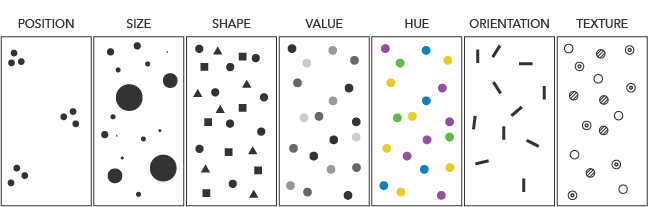
\includegraphics[width=\textwidth]{figures/related-work/visual-variables}
  \caption{Bertin's original visual variables~\parencite{Foster2017}.}
  \label{fig:related-work:visual-variables}
\end{figure}

\subsection{Choropleth maps}
Choropleth maps are thematic maps in which areas are shaded or patterned in proportion to the statistical variables being displayed on the map.
A popular use case is the display of population density or per-capita income.
An example of a choropleth map is shown in Figure~\ref{fig:related-work:choropleth}, visualizing the percentage of obese population in the US\@.
Choropleth maps are very popular and therefore many people are familiar with them already.
A downside of choropleth maps is that larger regions may appear more emphasized than smaller ones, since the entire area of regions is coloured.
Another disadvantage of choropleth maps is the common error of incorrect encoding:
Such an incorrect encoding would be the display of absolute numbers, e.g.\ total population or proceeds of crime, rather than relative numbers, e.g.\ population density or unemployment rate.

\begin{figure}
  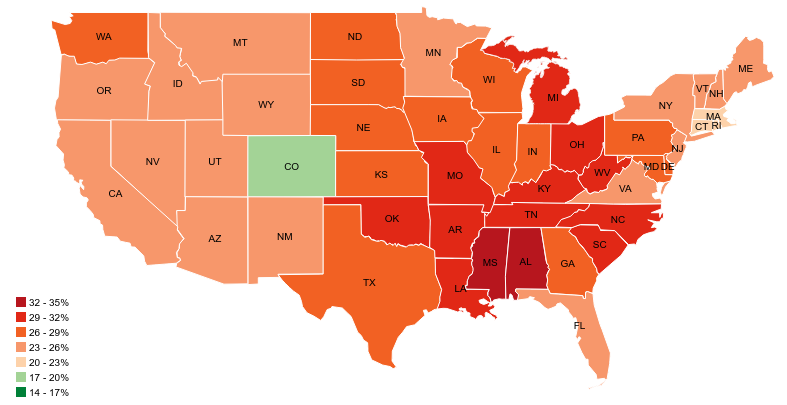
\includegraphics[width=\textwidth]{figures/related-work/choropleth}
  \caption{%
    Choropleth map of obese population, \gls{bmi} $ > 30 $, in the United States in 2008~\parencite{NCCDPHP2017}.
  }\label{fig:related-work:choropleth}
\end{figure}

\section{Information Visualization of Hierarchical Data}
The visualization of hierarchical data has a long tradition.
The traditional visual representation of a tree is a directed graph with the root node at the top, as seen in Figure~\ref{fig:related-work:tree-graph}.

An common use case is a directory tree of a file system, e.g.\ a file browser or the command line utility \texttt{tree} on UNIX based operating systems.
As \textcite{Shneiderman1992} mentions, this visualization becomes increasingly large when displaying more than one level and soon exceeds the entire screen size.

\begin{figure}
  \centering
  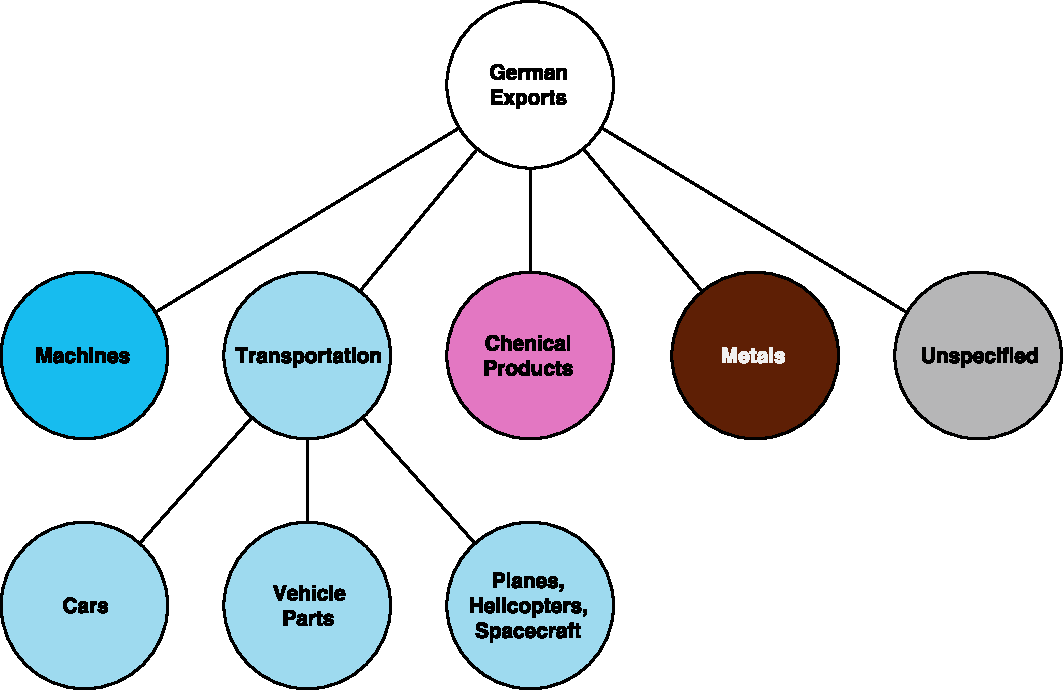
\includegraphics[width=0.6\textwidth]{figures/related-work/Treegraph}
  \caption{
    Traditional visualization of a tree in form of a directed graph with edges and nodes and the root node at the top.
    This example visualizes equivalently a part of the treemap visualization of German exports in Figure~\ref{fig:related-work:treemap-german-exports-1}.
  }
  \label{fig:related-work:tree-graph}
\end{figure}

\subsection{Treemaps}
\textcite{Johnson1991} propose the treemap visualization technique, in which each node is a rectangle whose area is proportional to a specified dimension.
In treemaps every node is visualized as a tile.
The membership relationship is expressed with tiles containing other tiles, thus representing the hierarchy.

Figures~\ref{fig:related-work:treemap-german-exports-1} shows an example of a treemap and Figure~\ref{fig:related-work:treemap-german-exports-2} shows the same treemap in another level of detail.
German exports are divided in generic groups like ``Machines'' and ``Chemical Products'' and include more specific groups like ``Cars'' and ``Packaged Medicaments''.
The user can click on a drop-down menu to change the current level of hierarchy, only leaf nodes are displayed at a time.

The advantage of treemaps is that they are space-filling visualizations, i.e.\ they make 100\% use of the available screen size.
A treemap will, unlike a graph representation of a tree, never exceed the size of the screen.

The area of the tiles can be mapped to a data attribute, e.g.\ the file size on disk or, in cases of Figures~\ref{fig:related-work:treemap-german-exports-1} and~\ref{fig:related-work:treemap-german-exports-2}, the percentage of export quota.
Thus, a treemap can display even more information than a traditional graph representation.
A disadvantage of treemaps is the variable size of each node.
If more and more nodes are displayed, the size of each tile will get smaller and smaller and e.g.\ there might not be enough space to display a label.
You can see this problem occur in Figure~\ref{fig:related-work:treemap-german-exports-2}.

\begin{figure}
    \centering
    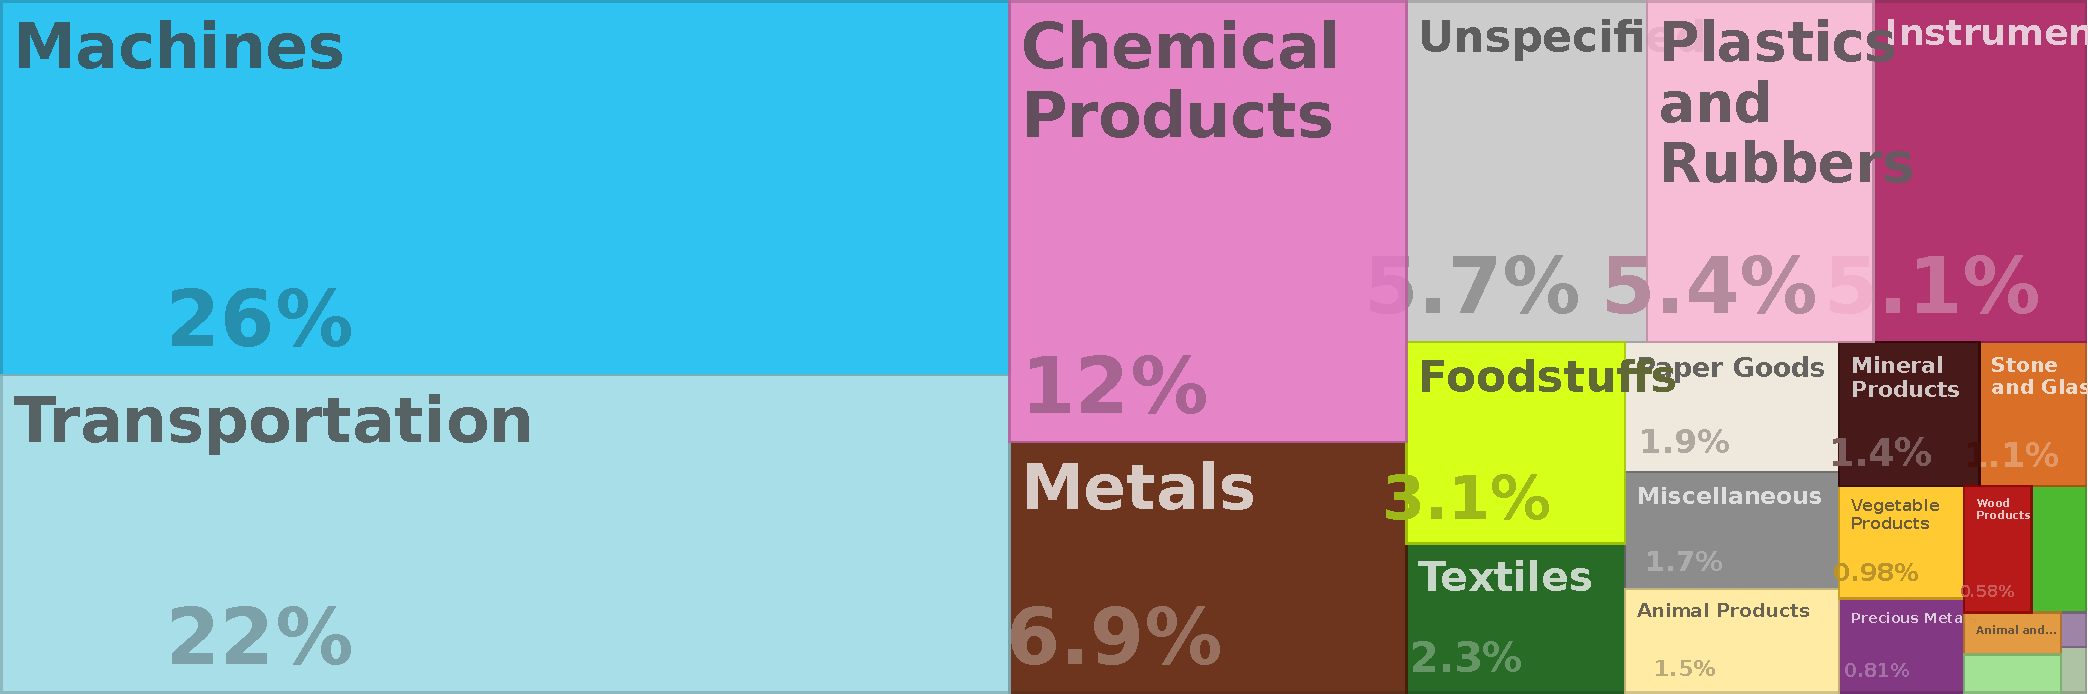
\includegraphics[width=\textwidth]{figures/related-work/en_profile_country_deu_1}
    \caption{A two dimensional treemap of Germany's foreign trade quota of exports, showing only the first hierarchy level~\parencite{Observatory2017}.}
    \label{fig:related-work:treemap-german-exports-1}
\end{figure}

\begin{figure}
    \centering
    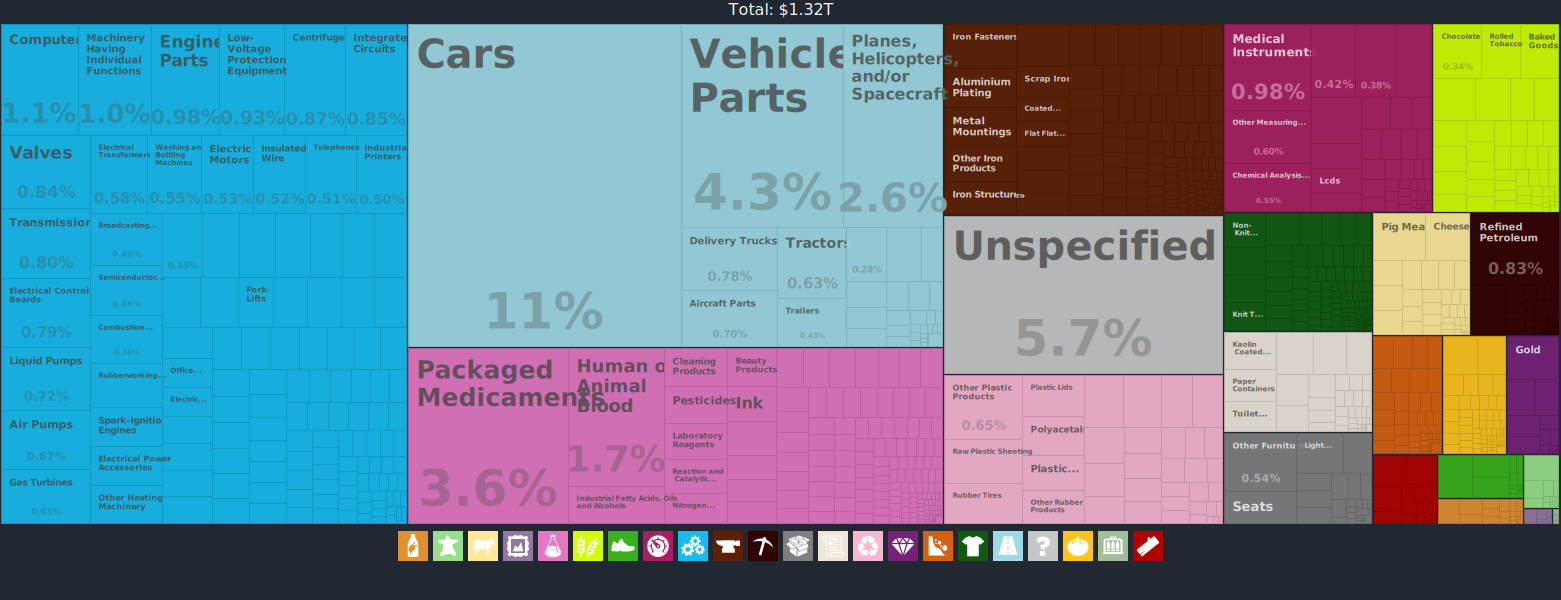
\includegraphics[width=\textwidth]{figures/related-work/en_profile_country_deu_2}
    \caption{Second level of detail of the treemap in Figure~\ref{fig:related-work:treemap-german-exports-1}~\parencite{Observatory2017}.}
    \label{fig:related-work:treemap-german-exports-2}
\end{figure}

If treemaps are used to visualize geographic data like municipalities, real estates or streets, the placement of nodes depends on the tiling algorithm and not the geographic location on a map.
Let's say a treemap visualizes a hierarchy of federal states and municipalities with the area of each tile mapped to the total population of administrative district.
Even if the membership hierarchy is matched by the treemap, the placement of districts in the same hierarchy level is based on their total population and not their geographic location.

\subsection{Spatially Consistent Treemaps}
When visualizing geographical data with a treemap, e.g.\ census data, it is desired to have a spatially consistent visualizations
The layout of hierarchical administrative subdivisions should approximately match a \gv{} of these subdivisions.
An early algorithm for geographically consistent treemaps is called ``Spatially Ordered Treemaps'' by \textcite{Wood2008}.
It is a modification of the ``Squarified Treemap Algorithm''~\parencite{Bruls2000}.
This modification places nodes based on their distance to the enclosing rectangle to be filled, rather than in the weight sequence order.
As \textcite{Ghoniem2015} demonstrate, this algorithm shows undesirable fragmentation for large, flat hierarchies.
One especially serious manifestation of this problem is visible in Figure~\ref{fig:related-work:spatially-ordered-treemap}.

Less fragmented but also less consistent regarding the geographic correctness are ``Histomaps'' by \textcite{Keim2002}.
This treemap algorithm sorts nodes such that their direction in the layout approximates their direction with regard to latitude and longitude.
This does not lead to fragmentation, but also does not guarantee geographic correctness.

\textcite{Ghoniem2015} developed ``Weighted Maps'' which are considered to be a trade-off algorithm for ``HistoMaps''.
This trade-off is between aspect ratio and geographic correctness.
Generally speaking, these treemap algorithms suffer because two unrelated circumstances are visualized in the same view.
For that reason, the approach in this paper is to establish the geographic context in a separate view and let treemaps excel in what they are best:
Visualizing hierarchical data.

\begin{figure}
  \centering
  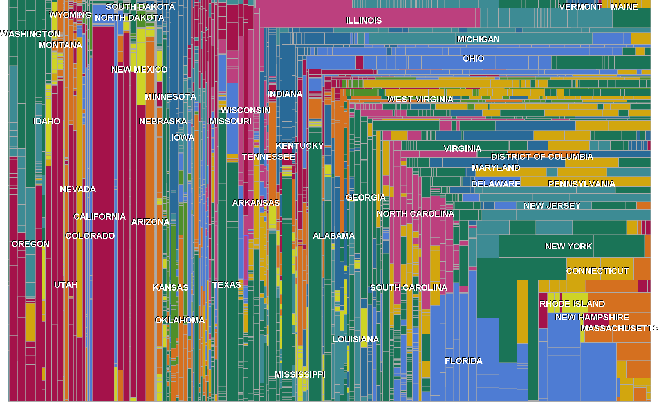
\includegraphics[width=\textwidth]{figures/related-work/spatiallyOrderedTreemap}
  \caption{
    A ``Spatially Ordered Treemap'' by \textcite{Wood2008} visualizing the population in 3,109 counties in the USA~\parencite{Ghoniem2015}.
    This algorithm shows severe fragmentation for large, flat hierarchies.
  }\label{fig:related-work:spatially-ordered-treemap}
\end{figure}


\subsection{3D treemaps and \tmaps{}}
3D treemaps are a concept introduced by \textcite{Bladh2004} in 2004.
The authors transfer the concept of treemaps from two dimensional into three-dimensional space, transforming tiles to blocks.
They introduce ``StepTree''~\parencite{Bladh2004}, which is a three-dimensional treemap to display a directory layout of a file system.
It ``differs from treemaps in that it employs three dimensions by stacking each subdirectory on top of its parent directory.''

3D treemaps are superior to 2D treemaps for tasks with a pronounced topological challenge.
Users perform significantly better in interpreting the hierarchical structure.
However, 3D visualizations also introduce some disadvantages.
Blocks can superimpose each other, forcing the user to navigate the view point.
The navigation of the view point itself is an increase of complexity not present in two dimensional treemaps.

The term \tmap{} was coined by \textcite{Limberger2016} in 2016.
A \tmap{} is just an ordinary 3D treemap, but it has all blocks attached to the ground, or more specifically, attached to the parent block.
An example of a \tmap{} is shown in Figure~\ref{fig:research:ua_treemap}.

\begin{figure}
  \centering
  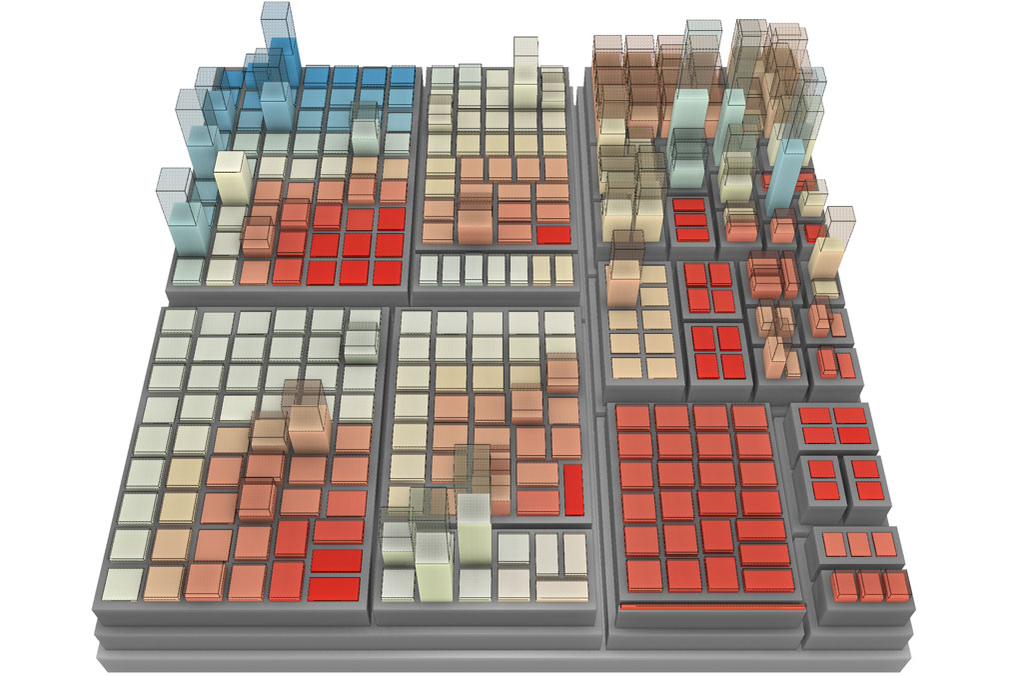
\includegraphics[width=\textwidth]{figures/related-work/2_5D_treemap_example}
  \caption{Example of a \tmap{}~\parencite{Doellner2017}.}
  \label{fig:research:ua_treemap}
\end{figure}

\section{Coordinated Multiple Views}\label{sec:related-work:cmvs}
\cmvs{} are a combination of data visualizations of the same data set in multiple views, often side-by-side.
According to \textcite{Roberts2007} \cmvs{} are just ``a specific exploratory visualization technique that enables users to explore their data.
The overall premise for the technique is that users understand their data better if they interact with the presented information and view it through different representations.''~\parencite{Roberts2007}

Some \cmvs{} are shown in Figure~\ref{fig:related-work:cmv}.
They display spatial and temporal attributes of pictures from a picture database as well as continuous attributes like popularity and number of comments.
The user can move the mouse cursor over each item in the scatter plot and the graduated symbol map and the corresponding item is highlighted with a larger stroke in all other views.
On the time line below, the user can also filter for pictures in a certain time frame by dragging the mouse from lower to upper limit.

\begin{figure}
  \centering
  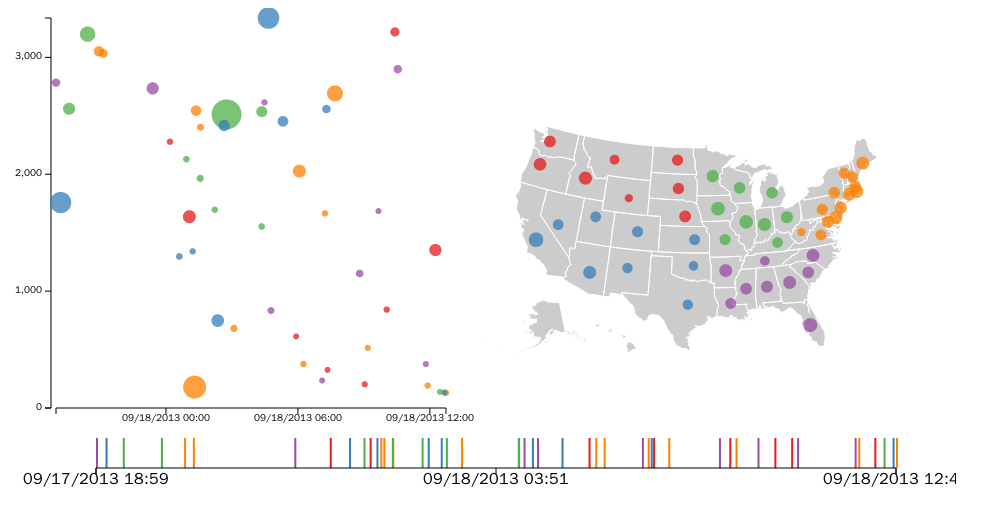
\includegraphics[width=\textwidth]{figures/related-work/cmv}
  \caption{\cmvs{} displaying the popularity, number of comments, location and time of pictures in a picture data base~\parencite{Dukevis2017}.}
  \label{fig:related-work:cmv}
\end{figure}

\subsection{Brushing and Linking}
Brushing and linking is a common interaction pattern found in \cmvs{} and often a crucial part of these visualizations.
``The technique of brushing is the principle approach, where elements are selected (and highlighted) in one display, concurrently the same information in any other linked display is also highlighted.''~\parencite{Roberts2007}

An example is given in Figure~\ref{fig:research:brushing-linking}.
It displays an on-time performance of airlines, visualized with the ``Crossfilter'' JavaScript library.

Each of the flight in the data set has an hour and a date for departure, an arrival delay, which can also be negative, and a traveled distance in miles.
The user can ``brush'' the data by selecting an interval by dragging the mouse.
The respective view will become a primary view and display the deselected items with a grey colour.

All other views become secondary views and display only selected items.
The visualization takes the most recent 80 flights from the database that match all given filters.
The user can further filter for items by dragging another interval in one of the secondary views.

This technique of propagating interactions to other views is called ``linking''.

Figure~\ref{fig:research:brushing-linking} shows a filter for travels with a long delay, i.e.\ from 120 minutes to the maximum value, see the selection in the upper center.
In the view in the upper left corner in Figure~\ref{fig:research:brushing-linking} long delays correlate with the time of the day.

\begin{figure}
  \centering
  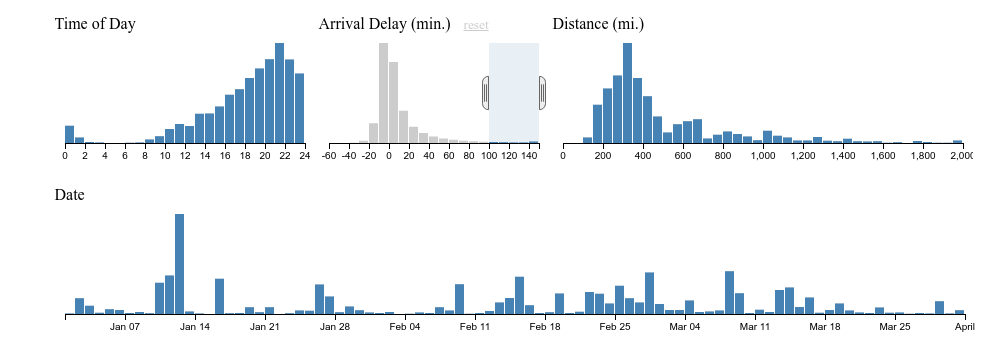
\includegraphics[width=\textwidth]{figures/related-work/brushing_linking}
  \caption{Airline on-time performance: Correlation of time of day with arrival delay. Most recent flight with a delay of more than 100 minutes selected~\parencite{Bostock2017}.}
  \label{fig:research:brushing-linking}
\end{figure}

\section{Modern Web Technologies}
This section introduces some state-of-the-art libraries, frameworks and standards for web development, as the existing \visan{} is a web application.
While not dedicated for \cmvs{} only, these technologies are either considered or used for the implementation of the additional \gv{}, as described in Chapter~\ref{sec:implementation}.

\textbf{CrossfilterJS} is one of the very few libraries dedicated for \cmvs{}.
It simplifies the implementation of brushing and linking interactions among several timeline visualizations of tabular data.
However, this library is unmaintained as of December 2017, the most recent commit dating back to March 2016.

\textbf{Leaflet} is the leading open-source JavaScript library for mobile-friendly interactive maps~\parencite{Leaflet2017}.
It has support for GeoJSON which makes it very easy to display tiled web maps with interactive overlays.

\textbf{Web components} is a recent standard of the \textcite{W3C2017} to bring component-based software engineering to the world wide web.
Web components are a set of web platform APIs to create new custom, reusable, encapsulated HTML tags that can be used in web pages and web applications~\parencite{WebComponents2017}.
Because of their encapsulation and reusability, web components are a promising choice for \cmvs{} that are implemented in JavaScript based web applications.

\textbf{ReactJS} is an open-source JavaScript library to build user interfaces and allows to create reusable UI components.
React renders HTML on the client, it changes the page without reloading the page.
The framework corresponds with the View in the Model-View-Controller pattern.
React components are structured hierarchically, with each component having dedicated responsibility.
React is explicitly not implementing web components and is not going to implement web components in the future.
It has, in return, a well-known way of integrating the component framework into a legacy application built with e.g.\ jQuery.

\textbf{GlimmerJS} is the rendering enginge of EmberJS~\parencite{Glimmer2017}.
In 2017 it was released as a standalone component framework.
Applications written in GlimmerJS can be exported as web components.
These web components can be included in any website, which makes GlimmerJS a reasonable choice to build high-quality widgets for user interfaces.

\textbf{Google Polymer} is another popular library to build web components~\parencite{Polymer2017}.
With 18,469 stars on Github it is the most popular framework for web components at the time of writing.
Polymer has a large community and comprehensive documentation and therefore more suitable than GlimmerJS to build \cmvs{}.


\textbf{PubSubJS} is a topic-based publish/subscribe library written in JavaScript~\parencite{PubSubJS2017}.
Topics can be registered hierarchically, with subtopics delimited by dots.
A subscription to topic \attr{mcv.select.focus} will be notified only for \attr{focus} interactions whereas a subscription of \attr{mcv.select} will be notified for both \attr{focus} and \attr{highlight} interactions.
Furthermore, topics are published asynchronously, so if the user interacts with a visualization, that does not block code execution.


\section{Related Work on Coordinated Multiple Views}\label{sec:related-work:guidelines}
The annual conference ``International Conference on Coordinated and Multiple Views in Exploratory Visualization'' provides a good selection of scientific papers in the area of \cmvs{}.
E.g.\ four papers of the conference of 2007 provide an introduction into the area of research:
``Coordinated Multiple Views: a Critical View'' by \textcite{Andrienko2007},
``State of the Art: Coordinated \& Multiple Views in Exploratory Visualization'' by \textcite{Roberts2007},
``The Future of CMV'' by \textcite{Erbacher2007} and
``Is coordination a means to collaboration?'' by \textcite{Weaver2007}.
Other papers present specific applications of \cmvs{} or user studies.
Relevant for this thesis are interaction aspects, in order to develop a conceptual framework of \cmvs{}, and guidelines for multiple views, to evaluate the system.

\subsection{Guidelines for Multiple Views}\label{sec:related-work:guidelines}
\textcite{Baldonado2000} established 8 rules as guidelines for multiple views.
These guidelines can be used to either choose a \cmv{} for an application or to improve the user experience for existing \cmv{} applications.
Each rule comes with a set of defined positive impacts on utility as well as negative impacts on utility.
Following these rules, designers and developers can tell whether the benefits of multiple views outweigh their drawbacks.

The eight rules are as follows:
\begin{enumerate}
  \item
    The rule of diversity: Use multiple views when there is a diversity of attributes.
  \item
    Complementarity: Use multiple views when different views bring out correlations or disparities.
  \item
    Decomposition: Partition complex data into multiple views to create manageable chunks.
  \item
    Parsimony: Use multiple views minimally.
  \item
    Space/Time Resource Optimization: Balance the costs of presenting multiple views with the benefits of using them.
  \item
    Self-Evidence: Use perceptual cues to make relationships more apparent.
  \item
    Consistency: Make the interfaces and states for multiple views consistent.
  \item
    Attention Management: Focus the attention of the user on the right view at the right time.
\end{enumerate}



\subsection{Interaction Aspects}\label{sec:related-work:interaction-aspects}
According to \textcite{Ho2013} interactions are a crucial part of data visualizations, yet most research in the area still focuses on visual representations.
Roughly speaking, research on interaction falls into these groups:
How to categorize interaction techniques?
How to find new interaction techniques and apply those to visualizations?

The following sections will give an overview of relevant research in interaction aspects for each group.

\subsubsection{Interaction Categories}\label{sec:related-work:interaction-aspects:categories}
This section covers high-level classification and categorization of interactions in \cmvs{}.

In 1996 \textcite{Shneiderman1996} classified interactions into six groups:
\begin{enumerate*}[label=(\arabic*)]
  \item
    Gain an \emph{overview} of the entire collection,
  \item
    \emph{zoom} in on items of interest,
  \item
    select an item or group and get \emph{details} when needed,
  \item
    view \emph{relationships} among items,
  \item
    keep a \emph{history} of actions to support undo,
  \item
    allow \emph{extraction} of sub-collections and of the query parameters.
\end{enumerate*}

Two years later, \textcite{Dix1998} identified these categories:
\begin{enumerate*}[label=(\arabic*)]
  \item
    \emph{Highlight and focus} particular subsets of the data,
  \item
    instead of displaying everything simultaneously \emph{access extra information} by drilling down the data,
  \item
    zoom in and out to give an \emph{overview and context},
  \item
    \emph{change parameters} of the \emph{same representation}, e.g.\ another baseline of a stacked bar chart,
  \item
    \emph{change representation} of the \emph{same data} by switching the chart type,
  \item
    \emph{link representations} to determine the relationship between items.
\end{enumerate*}

In 2002, \textcite{Keim2002} defined the following classification:
\begin{enumerate*}[label=(\arabic*)]
  \item
    Dynamic \emph{projection} to show all combination of data attributes mapped to the axis of a diagram,
  \item
    focus on a smaller subsets by \emph{filtering} out parts of the data,
  \item
    \emph{zoom} into a subset of the data and get a higher level of detail,
  \item
     drill-down operations to preserve an overview of the data are called \emph{distortion}
  \item
    and finally \emph{link and brush} visualizations, to highlight the same data points in multiple visualizations.
\end{enumerate*}

The most recent classification was done in 2007 by \textcite{Yi2007} listing seven categories:
\begin{enumerate*}[label=(\arabic*)]
  \item
    \emph{Select} to mark something as interesting,
  \item
    \emph{explore} to show something else,
  \item
    \emph{reconfigure} to show a different arrangement,
  \item
    \emph{encode} to show a different representation,
  \item
    \emph{abstract/elaborate} to show more or less detail,
  \item
    \emph{filter} to show something conditionally,
  \item
    \emph{connect} to show related items.
\end{enumerate*}

It is noticeable that all of these classifications of interactions are redundant.
E.g. there is a \emph{zoom} interaction for the first three classifications and all of them have a category similar to \emph{select}.
In this work the classification of \textcite{Yi2007} is used for the remaining parts because it is the most recent classification and it is based on the precursors.

\subsubsection{Formalization of Interactions}

This section covers the smaller part of research in \cmvs{}, research that is \emph{not} related to a high-level classification of interactions.
Not only interactions in \cmvs{} are considered but any kind of a formalization of interaction that may be used as the starting point for a framework for \cmvs{}.

\textbf{ITlib~\parencite{Figueroa2001}} is an architecture and a framework of interaction techniques for virtual reality applications, designed to be extensible and flexible.
New interaction techniques can easily be added and application specific code is seamlessly integrated.

On a low level an interaction technique ``is modeled as a set of filters connected in a small data flow''~\parencite[p.~2]{Figueroa2001}.
These filters are the smallest process unit in the data flow.
Composed of input and output ports, they communicate with other filters, to receive data input from predecessors and send data output to successors.

The framework specifies and stores the interaction techniques along with its filters, the execution model and the scene in \gls{xml} documents.

Even though the system describes interactions in an abstract way, the domain of the framework is clearly the interaction of a human body within a 3D virtual reality.
Certain assumptions are made, including the data model, which is the 3D scene, and human computer interaction devices, like the user's hand or the user's head.

The goal is not to better understand the data, which is the common goal in data visualizations.
In this case, the data model is the 3D scene and the goal is to manipulate the 3D scene.

Most importantly, the framework describes interaction techniques for a single viewpoint but not for coordinated multiple views.

\textbf{A framework for Focus+Context Visualization} by \textcite{Bjork1999} is one of the few formalizations of interactions in data visualizations.

The idea behind Focus+Context visualizations is to present the object of primary interest in full detail while at the same time giving a overview of the surroundings.

The authors of the paper distinguish visualizations and second-level visualizations:
Visualizations, referred to as $IV$, are triples of a set $[D]$ of underlying data, a visual representation $V$ and $I$ which is the possible interaction or manipulation.
\begin{equation}
  IV([D], V, I)
  \label{eq:focus-context:visualization}
\end{equation}
If $I$ affects $[D]$ the underlying data set can be manipulated.
Examples would be changes in a spreadsheet editor, or a change of the start and end date of an appointment in a calendar.

If $I$ affects $V$ the user can manipulate $IV$ in order to change the way $[D]$ is represented.
This statement holds e.g.\ for an interaction in which the user increases the visible level of hierarchy in a treemap.
According to \textcite{Yi2007} this would be an \emph{abstract/elaborate} interaction.
The effect of such an interaction is depicted by the change from Figure~\ref{fig:related-work:treemap-german-exports-1} to Figure~\ref{fig:related-work:treemap-german-exports-2} in Section~\ref{sec:related-work:cmvs}.

Second-level Visualizations are information visualizations consecutively applied.
The underlying data set $[D]$ of the formula in Equation~\ref{eq:focus-context:visualization} is replaced with some information visualization $IV$, which is compatible with $IV'$.
\begin{equation}
  IV'(IV, V', I')
\end{equation}

Focus+context visualizations are second-level visualizations.
An example given by the authors is the  ``rubbersheet'' visualization, that visually distorts a first-level visualization similar to a magnifier.
Regions of primary interest are distorted to appear magnified, while the remaining regions are minified.

The formalization of \textcite{Bjork1999} is suitable to describe multiple information visualizations applied one after another.
Yet, it is specialized on Focus+Context interactions.
It does not describe any kind of interaction in arbitrary information visualizations like line or bar charts.
This is also the reason why the formalization does not describe the exchanged data between views like identifiers of data points.


	\chapter{Analysis}\label{sec:analysis}
One purpose of this section is to abstract and deduce the essential characteristics of any interaction.
These characteristics are relevant for a formalized language of \cmvs{}.
To accomplish this goal, the approach is to deduce the characteristics by a list of examples.
What are the expected data structures for each visualization?
What visual variables can be used to show an interaction?
A list of possible interactions is given for each visualization.
Those interactions will be classified according to \textcite{Yi2007} and the relevant subject of the interaction is specified.

The second outcome of this section is a set of requirements which can be used to evaluate a framework of \cmvs{}.


\section{Single Visualization Interactions}\label{sec:analysis:examples:single}

The data visualization catalogue by Severino Ribecca list many of the most used data visualizations\cite{VisualizationCatalogue2017}.
This section covers a list of common data visualizations from that catalogue as examples.
The expected data structure and a list of possible interactions is systematically analysed.

\textbf{Line graphs}
\begin{figure}
  \begin{center}
    \subfloat[Line graphs]{{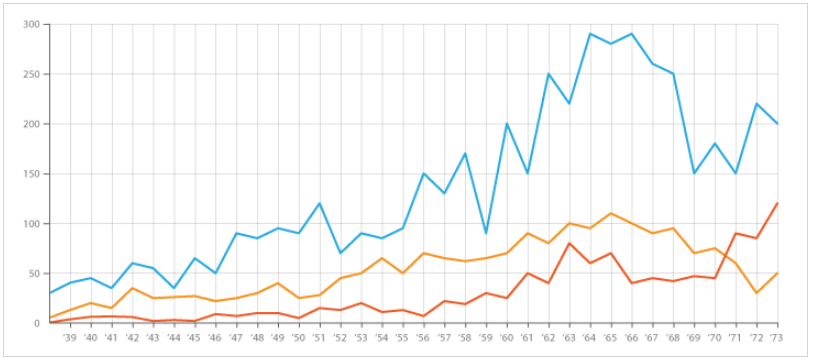
\includegraphics[width=0.4\textwidth]{figures/analysis/line-graphs} }}%
    \qquad
  \end{center}
  \caption{Line graphs are used to display trends}
  \label{fig:analysis:line-graphs}
\end{figure}

Line graphs display how quantitative values have changed over time.
They are perfectly suited to show trends or compare multiple series of data with each other.
The expected data format is \emph{tabular}, since one ore many series of data in parallel are visualized.

Line graphs are drawn in a Cartesian coordinate system, connecting subsequent points to each other.
Thus,
\begin{enumerate*}[label=(\arabic*)]
    \item position
    \item orientation and
    \item texture
\end{enumerate*}
are constrained by the nature of the visualization.
However, an interaction with the line graph can alter the
\begin{enumerate*}[label=(\arabic*)]
    \item shape
    \item color or
    \item size
\end{enumerate*}
of lines to create a visual effect.
It is further possible to highlight either the entire series of data or a single data point within that series, e.g. changing the shape and size of the point.
Table~\ref{tab:analysis:line-graph:interactions} shows a list of conceivable interactions in a line graph.

\begin{table}[H]
  \centering
  \caption{Interactions for line charts}%
  \label{tab:analysis:line-graph:interactions}
  \begin{tabular}{ll}
    \bf Select & Highlight a data point (id of data point) \\
    \bf Select & Highlight a data series (id of data series) \\
    \bf Encode & Change colours of data series (data series \rightarrow\ colour) \\
    \bf Filter & Restrict interval on x-axis (filter function of data attribute) \\
    \bf Filter & Hide a data series (id of data series) \\
  \end{tabular}
\end{table}




\textbf{Bar charts and multi set bar charts}

\begin{figure}
  \begin{center}
    \subfloat[Bar chart or column graph]{{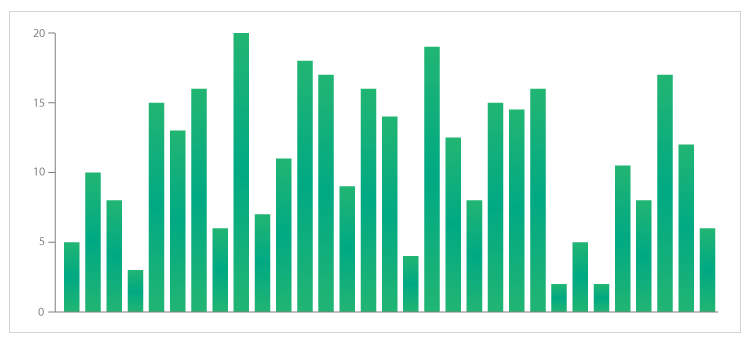
\includegraphics[width=0.4\textwidth]{figures/analysis/bar-chart} }}%
    \qquad
    \subfloat[Multi set bar chart]{{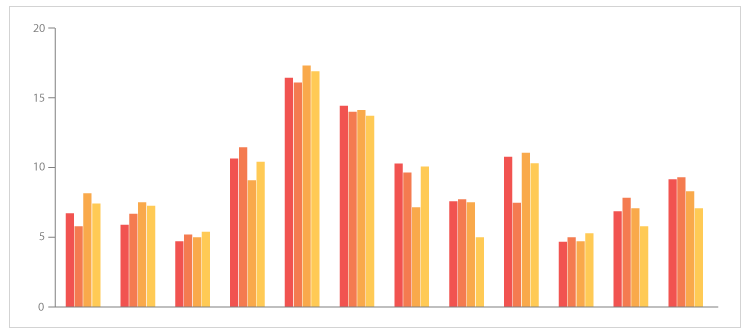
\includegraphics[width=0.4\textwidth]{figures/analysis/multiset-bar-chart} }}%
  \end{center}
  \caption{A multi set bar charts is a variation of a bar chart}
  \label{fig:analysis:bar-charts}
\end{figure}

Bar charts use either horizontal or vertical bars to show discrete, numerical comparisons across categories.
The length of a bar displays a quantitative value of a category.

Multiple bar charts display many data series next to each other.
Every series is grouped by category and a colour can be used to identify a data series.

Like line graphs, bar charts expect a \emph{tabular} data format.
In contrast to line graphs, bar charts are used to show a comparison rather than a trend.

The type of the visualization constrains the
\begin{enumerate*}[label=(\arabic*)]
    \item shape,
    \item size and, in case of a multi set bar charts,
    \item the colour
\end{enumerate*}
of the visualization.
An interaction can be shown by altering
\begin{enumerate*}[label=(\arabic*)]
    \item position,
    \item colour,
    \item shape and
    \item the texture
\end{enumerate*}
of bars and columns.
Table~\ref{tab:analysis:bar-charts:interactions} list some possible interactions.

\begin{table}
  \centering
  \caption{Interactions for bar charts}\label{tab:analysis:bar-charts:interactions}
  \begin{tabular}{ll}
    \bf Select & Highlight a bar (id of data point) \\
    \bf Encode & Change colours of data series (colours \rightarrow{} data series) \\
    \bf Reconfigure & Sort by attribute (data attribute) \\
    \bf Reconfigure & Drag bars to reorder data series (ordered list of ids of data points) \\
    \bf Filter & Hide a data series (id of data series) \\
  \end{tabular}
\end{table}

\textbf{Histograms}

\begin{figure}
  \centering
    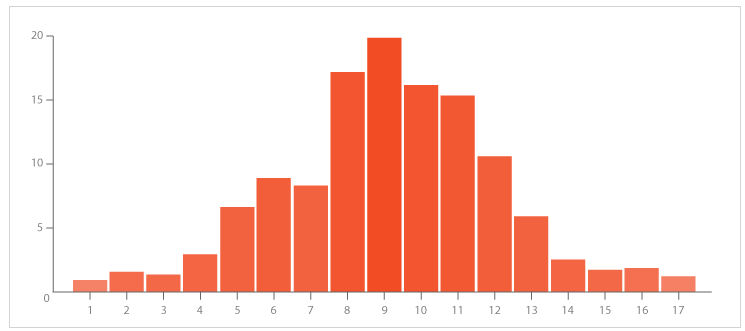
\includegraphics[width=0.4\textwidth]{figures/analysis/histogram.png}%
    \label{fig:analysis:histograms}
    \caption{A histogram is a bar chart over a continuous interval}%
\end{figure}

Histograms visualise the distribution of data over a continuous interval or certain time period.
A special type is the population pyramid, which is a pair of back-to-back histograms, one for each sex.
Histograms and bar charts expect the same kind of data, i.e.\ a \emph{tabular} format.
Almost the same interactions as in Table~\ref{tab:analysis:bar-charts:interactions} can be applied to histograms.
Except a re-ordering of bars along the x-axis, because the histogram constrains the position of bars along the interval.

\textbf{Bubble charts and scatter plots}

\begin{figure}
  \centering
    \subfloat[Bubble chart]{{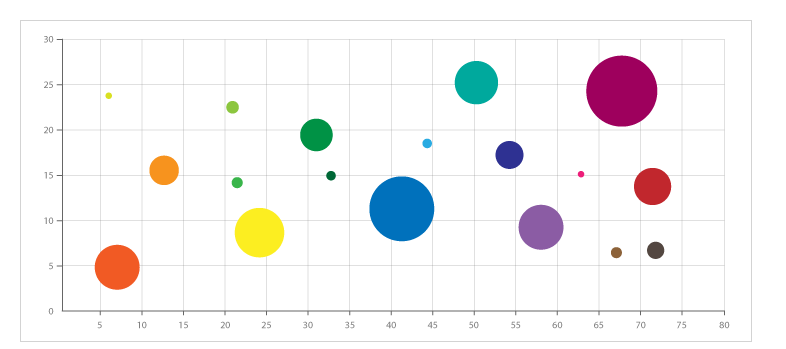
\includegraphics[width=0.4\textwidth]{figures/analysis/bubble-chart.png} }}%
    \qquad
    \subfloat[Scatter plot]{{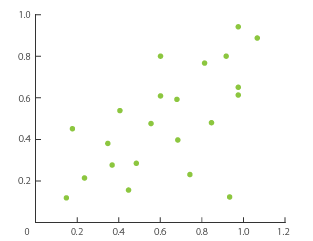
\includegraphics[width=0.4\textwidth]{figures/analysis/scatter-plot.png} }}%
    \caption{Bubble charts and scatter plots are similar regarding interactions}%
    \label{fig:analysis:bubble-chart}
\end{figure}

Both bubble charts and scatter plots are popular choices to visualize variables from two values.
Points are placed with the two values in Cartesian coordinates in order to detect relationships and correlations.
In case of bubble charts, each point is displayed as a bubble with a third value encoded in the size the bubble.
It is even possible to encode a fourth value in the colour of the bubble.

Like line graphs, bar charts and histograms, a scatter plot expects \emph{tabular} data.
Each data point can take up to four values (in case of a coloured bubble chart).
As we can see in Table~\ref{tab:analysis:bubble-charts:interactions}, interactions also include a zooming and movement of the viewpoint.
\begin{table}
  \centering
  \caption{Interactions for bubble charts}%
  \label{tab:analysis:bubble-charts:interactions}
  \begin{tabular}{ll}
    \bf Select & Highlight a bubble (id of data point) \\
    \bf Explore & Zoom in, zoom out (width and height of window) \\
    \bf Explore & Move viewpoint position (x- and y-coordinates of viewport) \\
    \bf Encode & Change mapping of colour to category (data series \rightarrow\ colour) \\
    \bf Encode & Change colour function (function value \rightarrow\ colour) \\
    \bf Encode & Change data attribute to colour (data attribute) \\
    \bf Encode & Change data attribute to size \\
    \bf Reconfigure & Sort by attribute (data attribute) \\
    \bf Reconfigure & Drag bars to reorder data series (ordered list of ids of data points) \\
    \bf Filter & Hide a data series (id of data series) \\
  \end{tabular}
\end{table}

\textbf{Stacked bar charts}

\begin{figure}
  \centering
    \subfloat[Stacked bar chart]{{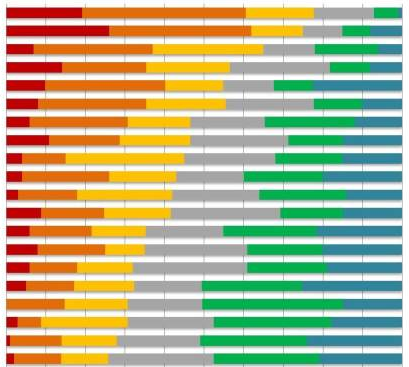
\includegraphics[width=0.3\textwidth]{figures/analysis/stacked-bar-without-baseline.png} }}%
    \qquad
    \subfloat[Stacked bar chart with baseline]{{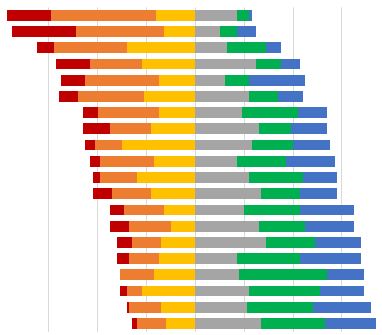
\includegraphics[width=0.3\textwidth]{figures/analysis/stacked-bar-with-baseline.png} }}%
    \caption{Stacked bar charts can be ordered along a baseline or stretch to 100\% width to show the percentage-of-the-whole of each group}%
    \label{fig:analysis:stacked-bar-chart}
\end{figure}
\begin{figure}
  \centering
    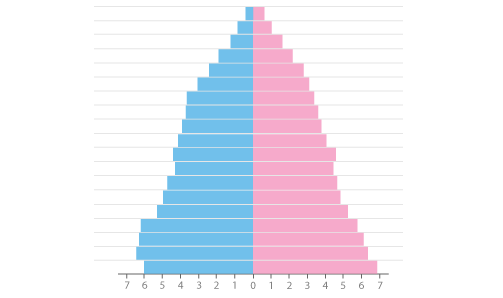
\includegraphics[width=0.4\textwidth]{figures/analysis/population-pyramid.png}%
    \label{fig:analysis:population-pyramid}
    \caption{A population pyramid can be modeled as a stacked bar chart}%
\end{figure}

Unlike a multi-set bar graph which displays their bars side-by-side, stacked bar graphs segment their bars of multiple datasets on top of each other.
A baseline, as shown in figure~\ref{fig:analysis:stacked-bar-chart} might be modeled as two back-to-back multi-set bar graphs. A reordering would e.g.\ move one data set from the left side to the right side.
A stacked bar chart also expects \emph{tabular} data
If the stacked bar chart has a baseline, often the sign of the numeric value defines the placement of the segment on the left or on the right side.
Table~\ref{tab:analysis:stacked-bar-chart:interactions} shows possible interactions, including the highlighting of a feature, a change of color mapping or a reordering of the baseline.
% \conceptTable{Tabular data, multiple date sets as series}{Size, shape, orientation.}{Color, position, texture.}

\begin{table}
  \centering
  \caption{Interactions for stacked bar charts}%
  \label{tab:analysis:stacked-bar-chart:stacked-bar-chart:interactions}
  \begin{tabular}{ll}
    \bf Select & Highlight a bar (id of data point) \\
    \bf Encode & Change mapping of category to colour (data series \rightarrow\ colour) \\
    \bf Reconfigure & Sort by attribute (data attribute) \\
    \bf Reconfigure & Reorder Y axis (ordered list of ids of data points) \\
    \bf Reconfigure & Sort stacking order by attribute (data attribute) \\
    \bf Reconfigure & Specify the stacking order data series (ordered list of ids of data series) \\
    \bf Reconfigure & Specify a negative data series (list of ids of data series) \\
    \bf Filter & Hide a data series (id of data series) \\
  \end{tabular}
\end{table}


\textbf{Hierarchical visualizations}

\begin{figure}
  \centering
    \subfloat[Tree map]{{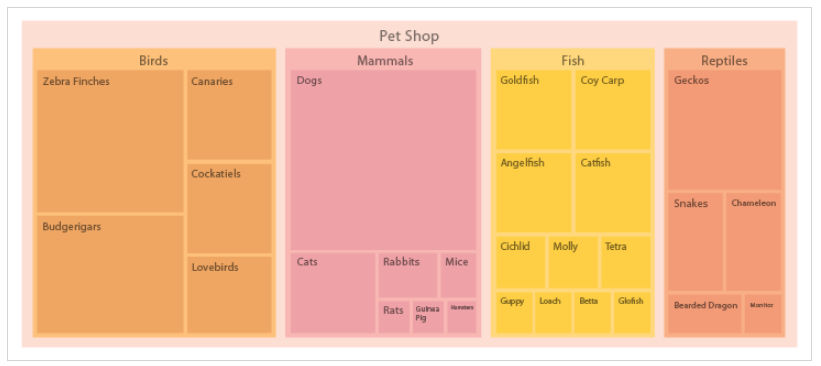
\includegraphics[width=0.4\textwidth]{figures/analysis/treemap.png} }}%
    \qquad
    \subfloat[Sunburst diagram]{{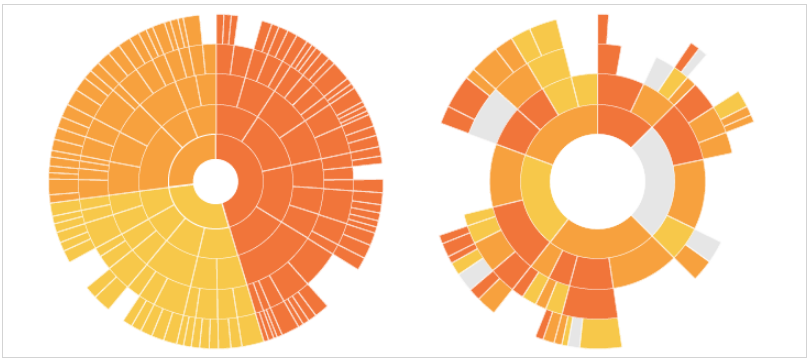
\includegraphics[width=0.4\textwidth]{figures/analysis/sunburst.png} }}%
    \caption{Tree maps and sunburst diagrams are ideal to show hierarchies}%
    \label{fig:analysis:hierarchies}
\end{figure}

Treemaps are great to show hierarchical data without ever exceeding the available screen.
Each feature is a assigned a rectangle according to a layouting algorithm.
Unlike a tree map a hierarchical ring diagram or sunburst diagram shows each level of the tree as a series of rings.

Therefore, both tree map and ring diagram expects \emph{hierarchical} data in form of a tree.
Each node needs to have at least one quantitative value for layouting, additionally, each node may be assigned a color.

As we are describing hierarchies, the maximal depth of tree may be increased or decreased.
Again, interactions could include a highlighting of features and a change of color encoding.
Both visualizations may show only a subtree.
E.g.\ a click on a box in the treemap opens another treemap focused on the subtree.
Similarly a click on a slice of the ring would surround the most external ring with the children of the feature.
Table~\ref{tab:analysis:hierarchies:interactions} gives a more comprehensive list of interactions.

% \conceptTable{Tree, each feature has a value for layouting.}{Position, Size, shape, orientation.}{Color, texture.}

\begin{table}
  \centering
  \caption{Interactions for hierarchical visualizations}%
  \label{tab:analysis:hierarchies:interactions}
  \begin{tabular}{ll}
    \bf Select & Highlight a feature (id of data point) \\
    \bf Explore & Use another node as root of the visible tree (id of data point) \\
    \bf Encode & Change mapping of category to colour (data series \rightarrow\ colour) \\
    \bf Reconfigure & Change data attribute used for layouting (data attribute) \\
    \bf Reconfigure & Sort by attribute (data attribute) \\
    \bf Reconfigure & Specify order (ordered list of ids of data points) \\
    \bf Abstract/Elaborate & Specify maximum depth of visible tree (number of levels) \\
  \end{tabular}
\end{table}

\textbf{Geographical Data}

\begin{figure}
  \centering
    \subfloat[Choropleth map]{{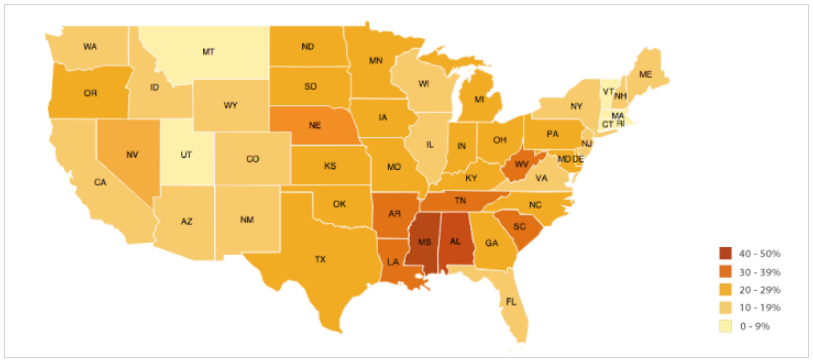
\includegraphics[width=0.4\textwidth]{figures/analysis/choropleth-map.png} }}%
    \qquad
    \subfloat[Flow map]{{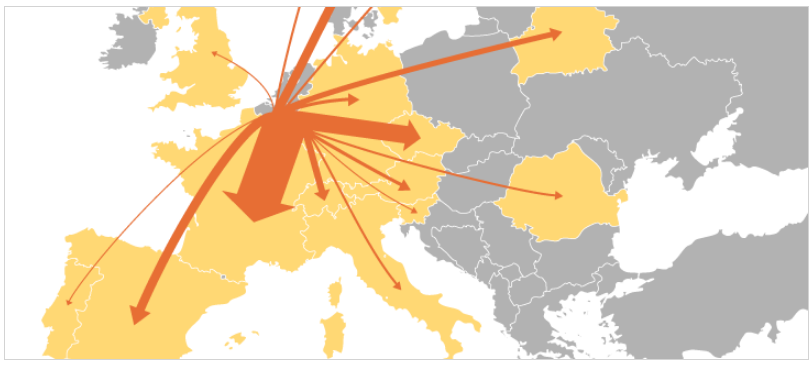
\includegraphics[width=0.4\textwidth]{figures/analysis/flow-map.png} }}%
    \caption{Choropleth maps focus on a density while flow maps show a migration of data}%
    \label{fig:analysis:geographical}
\end{figure}

Choropleth maps and flow maps are specialized diagrams focused on geographical data.
Size, position and shape of a feature is defined by the geometry data of a feature.
In choropleth maps the color of each feature is based on a data attribute.
Flow maps may display connections between features, a data value defining the size of each arrow.

Non-geographical data may be given in a \emph{tabular} form, assigned to each geographical feature.
In contrast to tabular data, a flow map expects relationships between geographical features.
Thus, it also expects \emph{relational} data in form of a graph

% \conceptTable{Graph data with edges, each feature has geometry data.}{Position, Size, shape, orientation.}{Color, texture.}

\begin{table}
  \centering
  \caption{Interactions for geographical visualizations}%
  \label{tab:analysis:geographical:interactions}
  \begin{tabular}{ll}
    \bf Select & Highlight a feature (id of data point) \\
    \bf Explore & Move viewport (latitude and longitude of viewport)\\
    \bf Explore & Zoom in, zoom out (zoom factor) \\
    \bf Encode & Change shape of marker (data id \rightarrow\ shape) \\
    \bf Encode & Change mapping of category to colour (data series \rightarrow\ colour) \\
    \bf Encode & Change colour function (value \rightarrow\ colour) \\
    \bf Encode & Change data attribute used for colour (data attribute) \\
    \bf Connect & Show relations of a feature (id of data point)  \\
    \bf Abstract/Elaborate & Change granularity of displayed regions (number of levels) \\
  \end{tabular}
\end{table}

\textbf{Activity diagrams}
\begin{figure}
  \centering
    \subfloat[Calendar]{{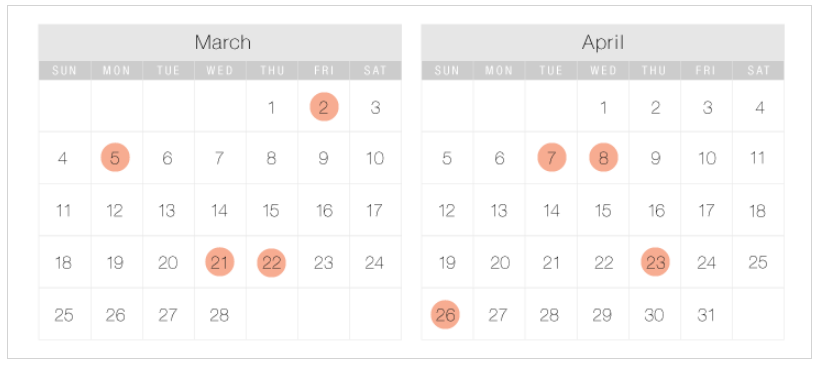
\includegraphics[width=0.4\textwidth]{figures/analysis/calendar.png} }}%
    \qquad
    \subfloat[Gantt chart]{{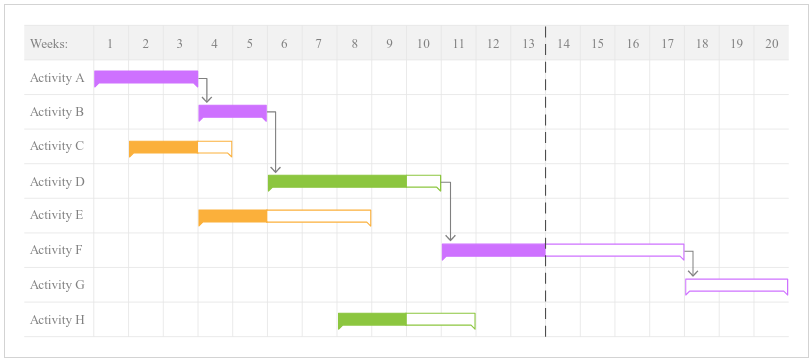
\includegraphics[width=0.4\textwidth]{figures/analysis/gantt-chart.png} }}%
    \caption{Similar to a calendar, a gantt chart shows activities and the progress along a time line}%
    \label{fig:analysis:temporal}
\end{figure}

In activity diagrams, each feature is represented as a rectangle, with the duration of the activity mapped to size and position.
Calendars and gantt charts could not only read the data from the data source, but also add new features to the data set or update metadata of a feature, e.g.\ the progress of the activity.
Calendars and gantt charts expect \emph{tabular} data, although data points might reoccur on a regular schedule.
So some data points, i.e.\ events, might repeat infinitely.

% \conceptTable{Temporal data, each feature has a time interval.}{Position, Size, orientation.}{Color, shape, texture.}

\begin{table}
  \centering
  \caption{Interactions for temporal visualizations}%
  \label{fig:analysis:temporal:interactions}
  \begin{tabular}{ll}
    \bf Select & Highlight a feature (id of data point) \\
    \bf Explore & Show a different period of dates (start and end datetime)\\
    \bf Explore & Show a different time interval (start and end hour)\\
    \bf Encode & Change color of categories or activities (data series \rightarrow\ colour) \\
    \bf Encode & Change data attribute used for colour (data attribute) \\
    \bf Filter & Remove a calendar or a category (id of data series) \\
  \end{tabular}
\end{table}

\section{Multiple View Interactions}\label{sec:analysis:examples:multiple}

\textbf{Detail view}
\begin{figure}
  \centering
  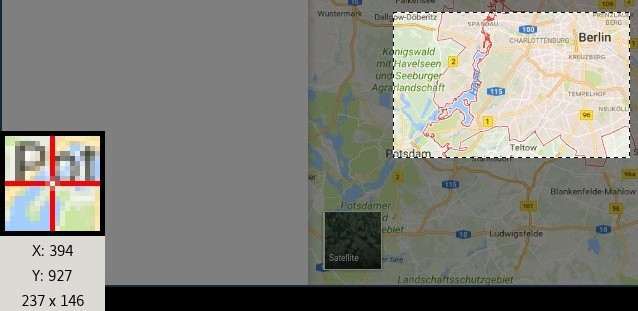
\includegraphics[width=0.4\textwidth]{figures/analysis/detail-view}
  \caption{The screenshot-tool ``shutter'' shows a magnified detail view of the area around the mouse cursor in the lower right corner of the screen}\label{fig:analysis:detail}
\end{figure}

\section{Requirements}
In this subsection, we list a set or requirements imposed on a \cmv{} framework.
These requirements can be used for further evaluation.
\textbf{Serialization} is the process of translating objects that can be stored or transmitted and reconstructed later.
In order to coordinate interactions among views, information needs to be passed from one view to another.
A framework for \cmvs{} should therefore find a serialization format for interactions which has
\begin{enumerate*}[label=(\arabic*)]
  \item
    small payloads and
  \item 
    fast serialization and deserialization.
\end{enumerate*}

\textbf{Reversibility} in the context of a \cmv{} framework means if it is possible to undo the effect of an interaction.
Ideally, every interaction function should have a well-defined inverse.
For every interaction that is not reversible, the computational cost to replay the interactions from the original state up to the point of the interaction should be minimal.

\textbf{Data extensibility} indicates the ease of reloading and updating data on the fly.
This is especially important if an interaction requests additional data from an external service.
We consider good extensibility when
\begin{enumerate*}[label=(\arabic*)]
  \item
    additional data attributes can be added without lookup of corresponding items and
  \item
    no de-duplication steps are necessary when new items are added.
\end{enumerate*}

\textbf{Development costs} qualify how much time and effort is needed in order to develop new components for the \cmv{} framework.
We track these costs in working days and the number of changed lines of code.


\textbf{Maintainability} means in our case, how much other views are impacted by a change of an interaction in one view and how error-prone the framework is.
In general it is hard to measure maintainability.
For the \cmv{} framework we want to measure the
\begin{enumerate*}[label=(\arabic*)]
  \item
    lines of code and the
  \item
    cycliomatic complexity. We will try to find a means to measure
  \item
    cohesion and
  \item
    coupling in the framework.
\end{enumerate*}
We assume that the amount of shared data between views is an indicator for high coupling.



\section{Comparison of client-side component frameworks}

This section evaluates the most suitable client-side rendering and component based JavaScript framework for \cmvs{} and whether or not to use web components.

Three JavaScript frameworks have been evaluated:
\begin{enumerate*}[label=(\arabic*)]
  \item GlimmerJS
  \item Google Polymer and
  \item ReactJS.
\end{enumerate*}
Google Polymer is built on top of web components and GlimmerJS applications can be exported as a web component, but React does not support web components.

\textbf{Web components} is a recent standard of the W3C\cite{W3C2017} to bring component-based software engineering to the world wide web.
Web components are a set of web platform APIs to create new custom, reusable, encapsulated HTML tags that can be used in web pages and web applications~\cite{WebComponents2017}.
If \cmvs{} are implemented in JavaScript based web applications, web components are a promising choice, to allow arbitrary views to be put together.


\textbf{GlimmerJS} is the rendering enginge of EmberJS\cite{Ember2017}.
In 2017 it was released as a standalone component framework.
Applications written in GlimmerJS can be exported as web components.
These web components can be included in any website, which makes GlimmerJS a reasonable choice to build high-quality widgets for user interfaces.
GlimmerJS also uses handlebars\cite{Handlebars2017}, a user-friendly templating language.
The downside of GlimmerJS is the current lack of documentation and immaturity due to the recent first release this year.

\textbf{Google Polymer} is another popular library to build web components \cite{Polymer2017}.
With 18,469 stars on Github it is the most popular framework for web components at the time of writing.
Polymer has a large community and comprehensive documentation and therefore more suitable than GlimmerJS to build \cmvs{}.

But critically, \cmvs{} require a means to exchange data between views, which is specific to interactions.
The web component specification, unfortunately, does not specify how arbitrary JavaScript objects can be passed to web components.
String based attributes are supported, as seen in Listing~\ref{lst:evaluation:web-components-data}.
To pass rich data to components however, web component frameworks have to roll their own data flow and syntax.
Google Polymer's syntax to pass rich data to a components is shown in Listing~\ref{lst:evaluation:polymer-data}.
But this is a proprietary solution that abandons standard HTML.

\lstinputlisting[
  language=HTML,
  label={lst:evaluation:web-components-data},
  caption={An example of string based attributes of web components~\cite{GoogleMapWebComponent2017}}
]{listings/evaluation/web-components-data.html}

\lstinputlisting[
  language=HTML,
  label={lst:evaluation:polymer-data},
  caption={An small syntax example how Google Polymer passes rich data to a component}
]{listings/evaluation/polymer-data.html}

This raises some problems in existing applications:
A particular component-based frontend framework can not be assumed, a lot of existing applications are also written without any JavaScript framework.
Proprietary solutions like the one of Polymer lessen the main motivation of implementing against web components:
Platform agnostic flexibility.

\textbf{ReactJS} is a JavaScript library for building user interfaces\cite{React2017}.
React is explicitly not implementing web components and is not going to implement web components in the future.
It has, in return, a well-known way of integrating the component framework into a legacy application built with e.g.\ jQuery.
Along with its major advantage of easy integration, it has a striving community, lots of documentation and tutorials and it is well tested.

As a summary, if there is
\begin{enumerate*}[label=(\arabic*)]
  \item no obligation to implement web components
  \item and an easy integration into an existing application is necessary,
\end{enumerate*}
then React is the perfect choice for \cmvs{}.
Figure~\ref{fig:implementation:frontend-frameworks} shows the pros and cons of each framework for the use case.


\begin{figure}[h!]
  \centering
  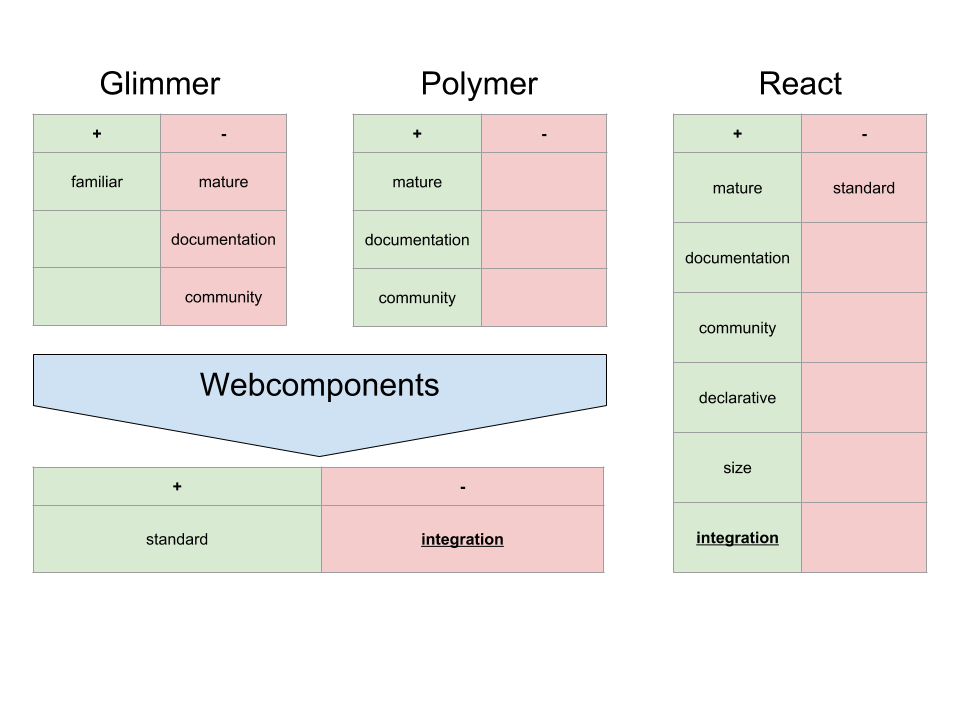
\includegraphics[width=\textwidth]{images/frontend-frameworks.png}
  \caption{Comparison of frontend frameworks}\label{fig:implementation:frontend-frameworks}
\end{figure}


	\chapter{Conceptual Framework}\label{sec:concept}
Based on the preparations in Chapter~\ref{sec:analysis:examples} this chapter specifies a conceptual framework for \cmvs{}.
The approach involves the definition of the terminology, a formalization of an interaction and the basic components of the conceptual framework.
These components are derived from the interactions and the data structures discovered in Chapter~\ref{sec:analysis}.

\section{The Conceptual Framework from the User Perspective}\label{sec:concept:framework}

Figure~\ref{fig:concept:component-diagram} shows a component diagram of the conceptual framework.
The user interacts via input devices, e.g. mouse or keyboard, with a computer.
In order to see the effect of the interaction the user oberserves an output device like a screen.

The computer or the browser provides an \gls{api} for these devices and the implementation of each view has access to this \gls{api}.
On the other side, views can communicate with each other through a coordinator.
This is necessary in order to coordinate interactions.

Each view can have multiple triggers and multiple effects.
A trigger is the handling of an event, caused by a user interaction, e.g.\ a mouse click.
A effect is the change of the visual representation of the view, in order to communicate the interaction.

Each view is self-responsible for the implementation of triggers and effects.
This is inevitable, as sometimes a view can not react to an interaction at all.
E.g.\ a re-ordering in a parallel plot will not affect a scatter plot, where the position of items is contrained by coordinates.

Interactions of the same category also need to be distinguishable.
E.g.\ the user could select a group of items with a bounding box.
Additionally, the user moves the mouse cursor on an item within that group in order to highlight the item.

Therefore the message exchanged between views not only includes the interaction category and the relevant item but also an interaction purpose.

Every view can subscribe to named interactions at the coordinator.
The coordinator notifies all subscribed views when a named interaction happens.
In order trigger an interaction, the visualization simply publishes the named interaction at the coordinator.
This pattern is known as the \emph{Publish-subscribe pattern} and widely used in message queues.


\begin{figure}[ht]
  \centering
  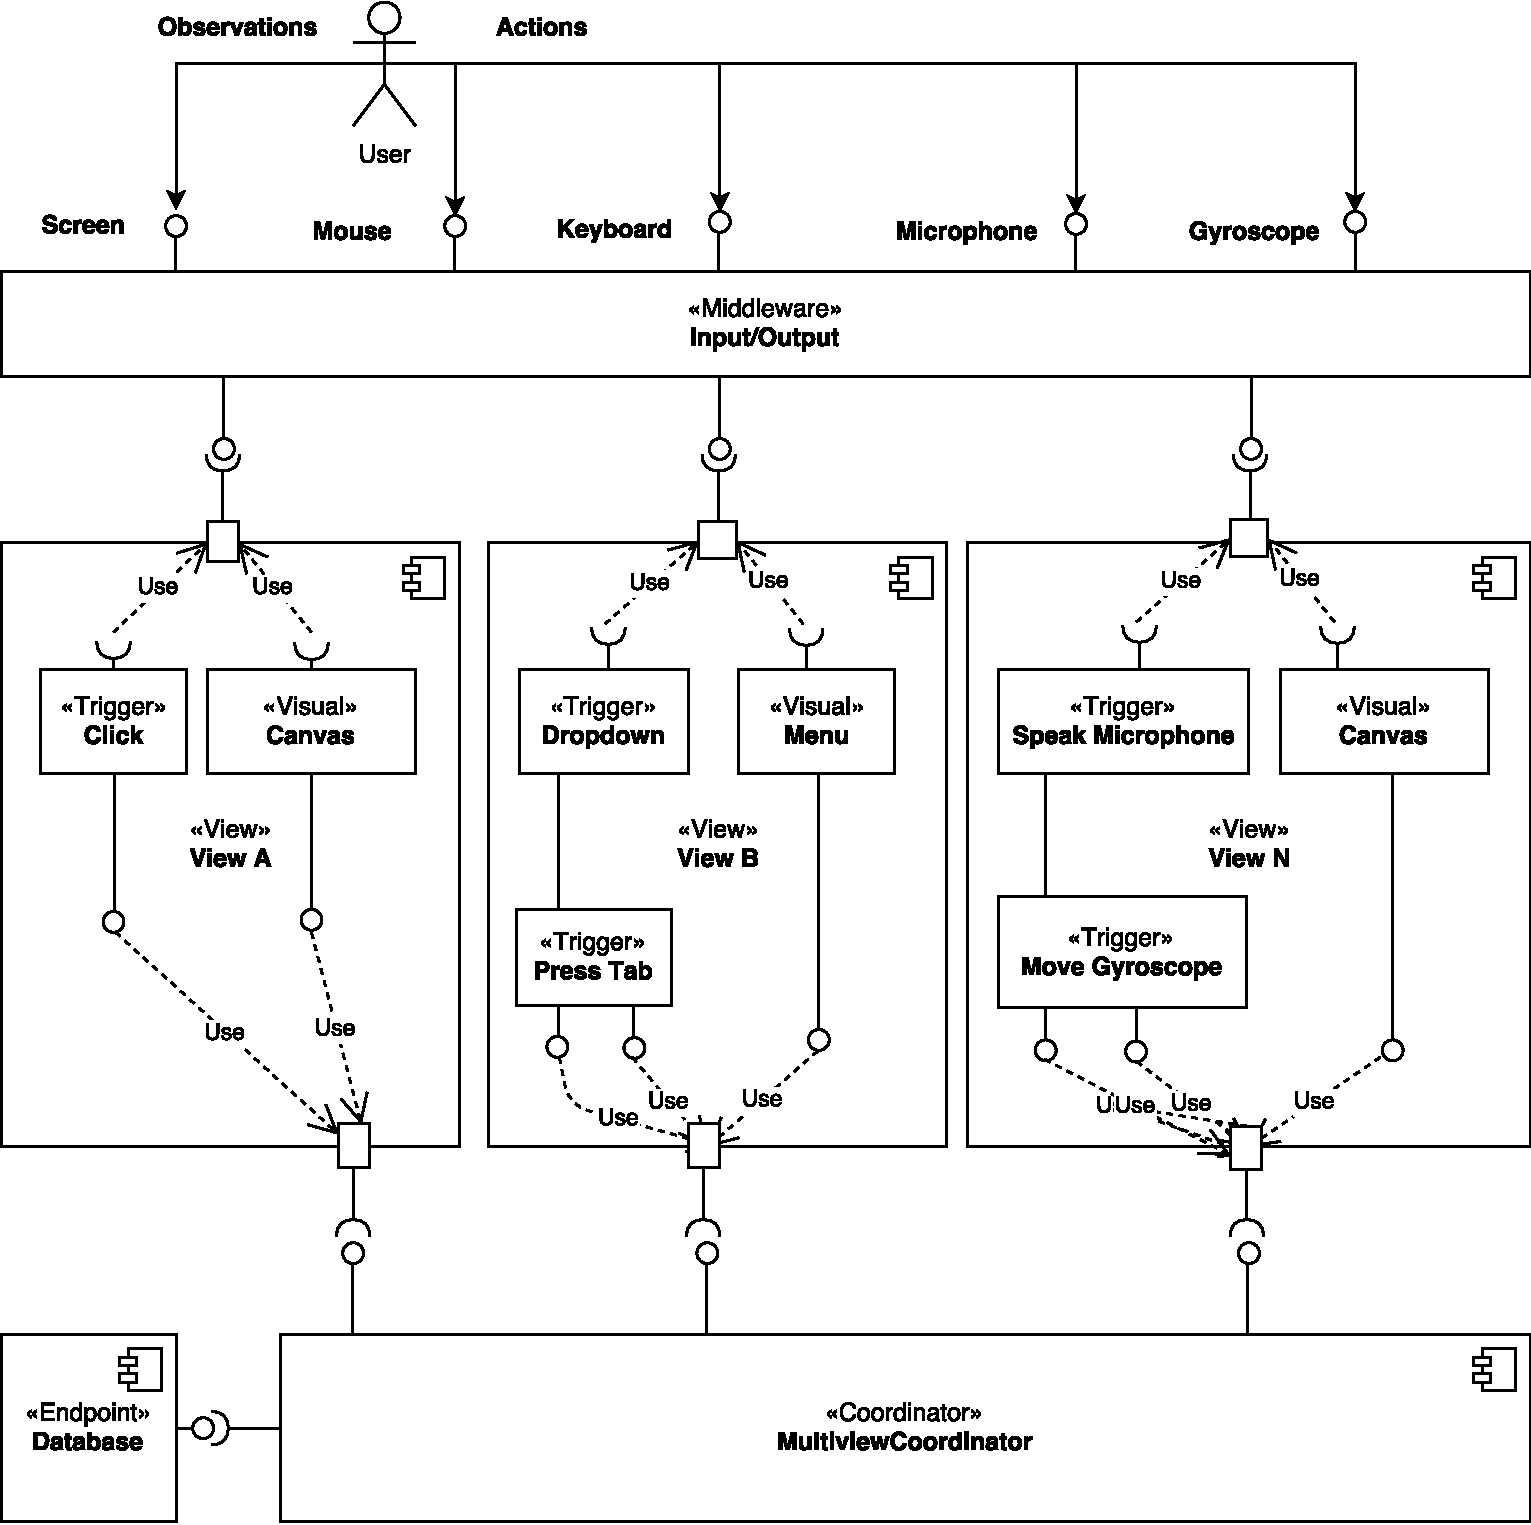
\includegraphics[width=\textwidth]{figures/concept/Concept}
  \caption{%
    Component diagram of the conceptual framework.
  }\label{fig:concept:component-diagram}
\end{figure}


\subsection{Interaction}
In single views, an interaction $I$ consists of at least a trigger and an effect:
\begin{equation}
  I(T, E)
\end{equation}
The purpose of the interaction in a single view does not need to be explicitly stated as such.
E.g.\ hovering over a geographic area changes the background colour of the polygon and the user can identify the interaction as a \emph{highlighting}.
This implicit meaning gets explicit in the described conceptual framework, so that views are able to react reasonably to interactions in other, outside views.

\subsection{Interaction in Coordinated Multiple Views}\label{sec:concept:framework:interaction}
An interaction $I$ in \cmvs{} is formalized as
\begin{equation}
  I(T, M(C,P,S), E)
\end{equation}
for a trigger $T$, a message $M$ and the effect $E$.
The message $M$ is defined by a category $C$, an application specific purpose $P$ as well as an interaction subject $S$.
The shared part of the interaction among multiple views is the message $M$.

\subsection{View}
A view is the section of the screen in which the user can see a data visualization.
A \cmv{} system shows multiple views, either side by side on a single screen or on different screens which are physically placed next to each other.


\subsection{Trigger}
If the event of a user action is handled by a view and causes an interaction, this handling is called a \emph{trigger}.
The user e.g.\ clicks on a shape in the view, hovers over an area, selects an item from a dropdown menu, turns around a mobile device, speaks into the microphone or makes a particular gesture.
As described in the introduction, views are responsible of their \emph{triggers}.


\subsection{Effect}
The effect is the change of the visual representation subsequent to the interaction.
In order to be perceivable by the user, the interaction must have some visual effect, e.g.\ a change of a visual variable according to \textcite{Bertin2010}.

Some examples are:
A change of colour of a selected bubble, a movement of the viewpoint, a rearrangement of attributes in a parallel plot or a higher level of detail in a \tmap{}.

Similar to a \emph{trigger}, a view is self-responsible of its visual \emph{effects}.
Obviously visual effects are not shared, as a visual variable might be constrained due to the nature of the visualization technique itself.
A re-ordering interaction in a parallel plot will not have an effect in bubble charts, as position is constrained by the type of visualization.

\subsection{Category}
An category is the declaration and definition how the subject of the interaction should be changed.
The aforementioned explicit meaning of the interaction is the smallest unit of information of the interaction.
Some examples of categories include: Selection, Deletion, Point-of-Interest, Filtering, Reordering, Re-encoding.
Categories can be classified with the interaction categories of \textcite{Yi2007}.

\subsection{Purpose}
The \emph{purpose} describes the interaction in the context of a task or an application specific intention.
A developer may want to have many \emph{select} interactions.
E.g.\ the user desires to select a detail view of an item under the mouse cursor from a previously selected set of already highlighted items.
Therefore two interactions of the same category can be distinguished by a user-defined \emph{purpose}.

\subsection{Subject}
A subject refers to the target of the interaction.
We must define what data or meta-data is affected by the interaction.
E.g.\ when a user moves the mouse cursor on a line in the line diagram, that could highlight the \emph{data point} under the cursor as well as the entire \emph{data series}.
Therefore we call the object affected of an interaction the interaction \emph{subject}.
A subject can be a data point, a list of data points, a position of the viewpoint, a certain order of attributes or a mapping of attributes to visual variables.



\section{Shared data model}\label{sec:concept:data-model}
The shared data model is a model of the data on which all visualizations must agree on.
To account for various data structures discovered in Chapter~\ref{sec:analysis}, we use an abstract data model that is inclusive enough to include tabular, hierarchical and relational data.
You can see a class diagram of this data model in Figure~\ref{fig:concept:shared-data-model}.

The \emph{entity} class is used to model the smallest distinguishable unit.
All entities can be identified and retrieved via the \emph{id}.
An entity is defined to be any object that can have data attributes attached as \emph{dimensions}.

While entities describe what an object \emph{is}, a \emph{dimension} describes what it \emph{has}.

An entity can have arbitrary many attributes and each value can be accessed by the name of the attribute.
So if you want to get the \emph{latitude} value of an entity, you can retrieve the value with a call to the dimension \emph{latitude}.

Entities can also be \emph{series} of other entities.
A series contains an ordered list of contained entities.
As series can also contain other series, so we can model a hierarchy relation.

Every entity has a \emph{parent} which is the series it is contained in.
The root entity of the hierarchy has a parent which is \attr{nil}.
Every series has a special attribute \attr{height} that describes the number of nested series or the height of the subtree.

If we just want to display tabular data, we just have one or two levels of hierarchy.
E.g.\ one level of hierarchy for a histogram and two levels of hierarchy for a stacked bar chart.

Other relations than hierarchical relations can be modeled as a \emph{relation} entity.
It represents a directed edge in a graph and must have incoming and outgoing entity.
Since every \emph{relation} is an \emph{entity} as well, we can add \emph{attributes} to the relation.
These attributes may describe e.g.\ the weight of an edge in a flow map.

\begin{figure}[ht]
  \centering
  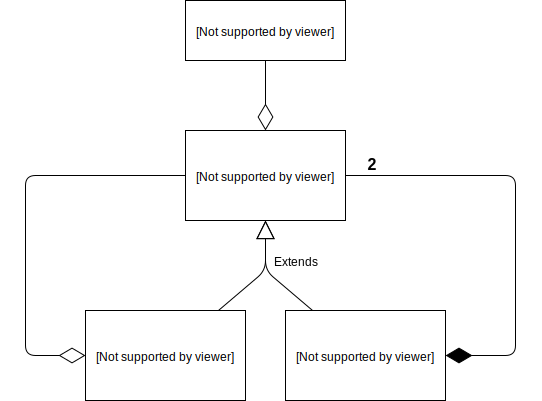
\includegraphics[width=\textwidth]{figures/concept/DataModel}
  \caption{%
    A data structure for tabular, hierarchical and relational data.
  }\label{fig:concept:shared-data-model}
\end{figure}



\section{Encoding of Interaction Subjects}\label{sec:concept:message-interface}

As described in Section~\ref{sec:concept:framework:interaction}, a message consists of the interaction \emph{category}, \emph{purpose} and \emph{subject}.
Category and purpose are just identifiers and can be encoded as a number or a string.
The subject is a highly variable object.
It could define some state, e.g.\ explicitly stating the id of an entity or the name of an attribute.
Alternatively, it could define some behaviour, e.g.\ implicitly defining if an entity is filtered based on its dimensions.
Therefore, the approach in this thesis is to model the subject as a mathematical function.
If the function has no input parameter, it just returns some state, i.e.\ the ids of \emph{entities}, \emph{series}, and \emph{relations} or their respective \emph{attributes}.
If the function depends on input parameters, it may return e.g.\ \attr{true} or \attr{false} or define a sort order.

In this section, a couple of function declarations are derived from the examples in Section~\ref{sec:analysis:examples}.
Domain and range of these functions refer to the objects defined in the data model in Section~\ref{sec:concept:data-model}.

\subsection{Set definitions}
The set of all entities $E$ in our subject space is defined as:
\begin{equation} \mathbb{E} : \mathbb{E} \subseteq \mathbb{N}  \end{equation}
Each entity can be represented by its \attr{id}, so for simplicity $\mathbb{E}$ is a subset all natural numbers in $\mathbb{N}$.

The set of all dimensions $D$ in our shared data model is defined as:
\begin{equation} \mathbb{D} : \mathbb{D} \subseteq \Sigma^* \end{equation}
For simplicity, each dimension is represented as a sequence of characters, with the set of all sequences of characters written as $ \Sigma^*$.

The set of all values of a dimension $d$ is defined as:
\begin{equation} Space(d), d \in \mathbb{D} \end{equation}
So for an attribute \attr{name}, $Space(name)$ would be the set of all strings.

Visual variables according to \textcite{Bertin2010} as in in Section~\ref{sec:related-work:visual-variables} are defined as:
\begin{equation} \mathbb{V} = \{position, size, shape, value, hue, orientation, texture\} \end{equation}


\subsection{Function declarations}
The functions $Select$ and $Filter$ operate on entities and can be used interchangeably:
\begin{equation}
\begin{split} Select: \varnothing \rightarrow \mathcal{P}(\mathbb{E}) \end{split}\qquad
\begin{split} Filter: \mathbb{E} \rightarrow \{ \bot, \top \} \end{split}
\end{equation}
  The empty set is written as $\varnothing$ and the set of all subsets of $E$ is written as $ \mathcal{P}(\mathbb{E})$.

  $Select$ just returns a subset of entities explicitly and expects no input.
  It can be used to highlight or focus entities, mark them for deletion or show details of an entity.

  $Filter$ returns for every entity either \attr{true} or \attr{false}, depending on the entity and the value of its dimensions.
  Instead of an explicitly defined set of filtered entities, entities are defined implicitly.
  A good example would be a filter function checking upper and lower limit for each entity and a dimension called \attr{price}.

\begin{equation}
\begin{split} Order: \varnothing \rightarrow \mathbb{E}^* \end{split}\qquad
\begin{split} Sort:  \mathbb{E} \times \mathbb{E} \rightarrow \mathbb{R} \end{split}
\end{equation}

  The functions $Order$ and $Sort$ are used to order two entities $e1, e2 \in \mathbb{E}$.
  The following equivalencies hold for $Sort$:
  \begin{align*}
     e1 < e2 \quad\Leftrightarrow\quad Sort(e1,e2) < 0 \\
     e1 = e2 \quad\Leftrightarrow\quad Sort(e1,e2) = 0 \\
     e1 > e2 \quad\Leftrightarrow\quad Sort(e1,e2) > 0
  \end{align*}

  Similar to $Select$ and $Filter$, these order functions can be implemented either explicitly or implicitly.
  $Order$ explicitly returns a sequence of entities, e.g.\ $(e4, e2, e5, e1, e3)$.
  $Sort$ implicitly orders two entities $e1$ and $e2$ based on their dimensions.
  E.g.\ ordering entities based on the alphabetical order of their name would be an example of the latter.

\begin{equation} Encode: \mathbb{D} \rightarrow \mathbb{V} \end{equation}
  The $Encode$ function can be used to change the mapping of dimension to a visual variable.
  E.g.\ bar charts, line diagrams, histograms and bubble charts can change the dimension mapped to their coordinate axes.
  Bubble charts can encode a different dimension in the \attr{size} of the bubbles.
  Choropleth maps, treemaps and bubble charts can map a different attribute to \attr{colour}.
  A specialized version of this function may return the attribute that is used for the layout algorithm in treemaps.

\begin{equation} Window: \mathbb{D} \rightarrow W, \quad W = \{w | w \subseteq Space(d), d \in \mathbb{D}\} \end{equation}
  For each of the dimensions in $\mathbb{D}$, the function returns the currently visible subset.
  E.g.\ a zooming or panning operation in a \gv{} would result in a change of \attr{latitude}, \attr{longitude} and \attr{zoom} of the viewpoint and therefore the currently visible section of the geographic vector space.
  The subset $w$ can be encoded implicitly or explicitly.
  For continuous values two representatives \attr{from} and \attr{to} could define an interval.
  E.g.\ in a calendar we map \attr{fromDay}, \attr{toDay}, \attr{fromHour} and \attr{toHour} to define the currently visible time section.
  If a dimension has discrete values, subset $w$ could also be encoded with all values explicitly stated.


% Let's have some examples how these functions can be applied on coordinated interactions:

% A user clicks on a bar in a bar chart and this feature then changes its background colour.
% To coordinate the highlighting, the bar chart view will formulate a new message composed of a \emph{Select} function and the category \emph{highlight}.
% The function returns the set with the highlighted entity.

% Let's say, a geographical map should move the position of the viewpoint on a entity.
% The triggering view will use a function \emph{Select} this time with a category \emph{focus}.
% A treemap as a third view could pick up that interaction and show a subtree with the focused entity as root node. 

% A view may show some controls to filter the data set, e.g.\ two sliders on an attribute called \attr{prize}.
% When the user releases the mouse, an interaction with the function \emph{Filter} and the category \emph{Hide} will be triggered.  
% The function will then check the \attr{prize} of every entity and returns \attr{true} if the prize is within the given lower and upper limit, \attr{false} otherwise.



	\chapter{Implementation}\label{sec:implementation}


This section describes the reference implementation for the conceptual framework in Chapter \ref{sec:concept}.
First, the general architecture is explained.
Various components and interaction techniques of the geographical visualization are detailed.
The integration of the geographical visualization in the existing \visan{} is shown.
The connection of the conceptual framework and the implemented framework is examined.

\section{Implemented interactions}

In the course of this thesis the following interactions have been implemented:
\begin{itemize}
  \item
    Select

    \begin{itemize}
      \item
        Highlighting an entity is possible by moving the mouse cursor on a geographic feature in the \gv{} or a block in the \tmap{}.
        The corresponding block or geographic feature will be highlighted respectively.
      \item
        A click on a block in the \tmap{} selects this entity in the \gv{} and vice versa.
      \item
        Holding the control key, multiple clicks on a block in the \tmap{} creates a group of selected entities.
        Corresponding geographic feature or blocks in the \tmap{} or \gv{} are selected as well.
    \end{itemize}

  \item
    Explore

    \begin{itemize}
      \item Selecting a block in the \tmap{} centers the viewpoint in the \gv{} on the corresponding geographic feature.
      \item Selecting a group of blocks in the \tmap{} centers the viewpoint in the \gv{} on the boundaries of all corresponding geographic features.
    \end{itemize}

  \item
    Reconfigure

    \begin{itemize}
      \item
        Choosing a different data set updates the geometries in the \gv{}.
      \item
        Selecting another shape for the \tmap{} (e.g. point instead of polygon geometries) changes the visual representation in the \gv{}.
    \end{itemize}

  % \item
  %   \emph{Filter}: The user double-clicks on a region in a geographical map and the \tmap{} will be based on data of only that region.
\end{itemize}
\todo[inline]{If we still have time, add filter interaction here}

\section{Coordinated Multiple View Layout}

Figure~\ref{fig:implementation:layout} shows the layout of the different views from the user perspective.
The \tmap{} is on the left, the \gv{} is on the right and some additional views to inspect and manually publish messages are displayed.

The currently visualized data set is called ``Wahlkreise'' and consists of German administrative districts.
The \tmap{} is tiled based on unemployment rate and the colour is based on the percentage of high-school graduates.
District ``Magdeburg'' is selected in the \gv{} with an unusually high percentage of graduates compared to other districts with a similar unemployment rate.

\begin{figure}[ht]
  \centering
  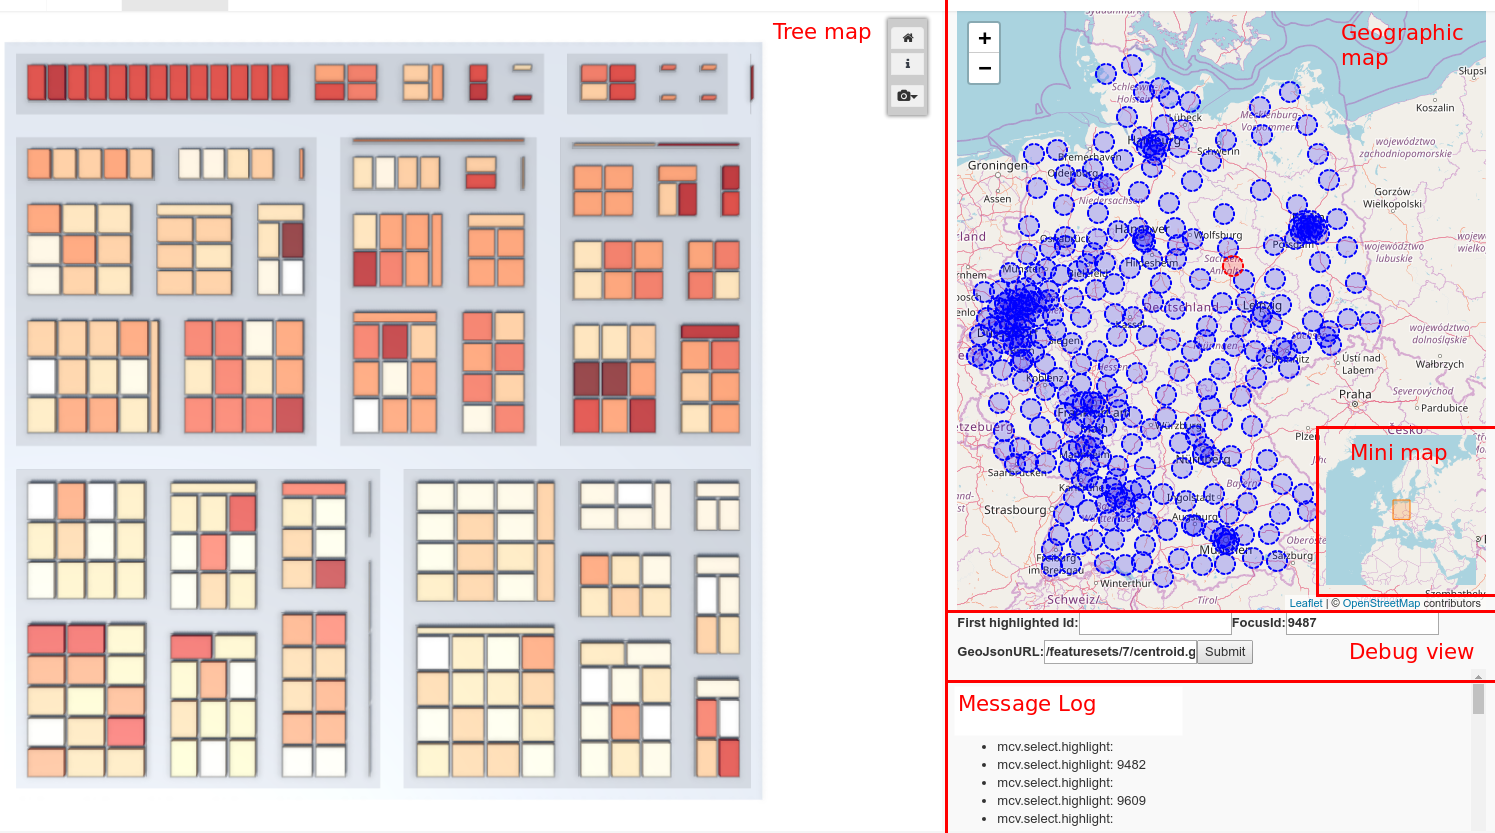
\includegraphics[width=\textwidth]{figures/implementation/Layout}
  \caption{%
    This Figure shows the layout of the \cmv{}, red lines indicate the borders of different views.
  }\label{fig:implementation:layout}
\end{figure}


\section{Architecture}
The architecture of the implementation is depicted in the class diagram in Figure~\ref{fig:implementation:architecture}.
For each of the views in Figure~\ref{fig:implementation:layout} you can see a corresponding class in Figure~\ref{fig:implementation:architecture}, i.e.\ \attr{Treemap}, \attr{MapComponent}, \attr{MessageLog} and \attr{DebugView}.

All views have a reference to \attr{MultiviewCoordinator} in order to subscribe to interactions.
The rendering \tmap{} is controlled by \attr{UAController}, thus it is connected to \attr{MultiviewCoordinator} through this class.
The \attr{MultiviewCoordinator} itself does not have a visual representation.

\subsection{Update mechanisms}
In Figure~\ref{fig:implementation:architecture} views with a \attr{render} are implemented as React components and can be rendered in place of a node inside the DOM tree.
React components and their dependant components get automatically re-rendered if their internal state changes.

E.g. if the position of the view point of the \attr{MapComponent} changes, that will re-render the included \attr{Map} which depends on the position.
If the Geometries of the visualized data set are updated, that will change the \attr{GeoJSON} component but not the \attr{Map}.

% Views implemented with React are dependency free except for a reference to a \attr{MultiviewCoordinator}.
% This makes those classes very easy to test.


\begin{figure}[ht]
  \centering
  \caption{%
    Architecture of components.
    Every class with a \attr{render} method is a React component.
    \attr{MultiviewCoordinator} is used to coordinate \tmap{} and \gv{} as well as to load geometry data.
  }\label{fig:implementation:architecture}
  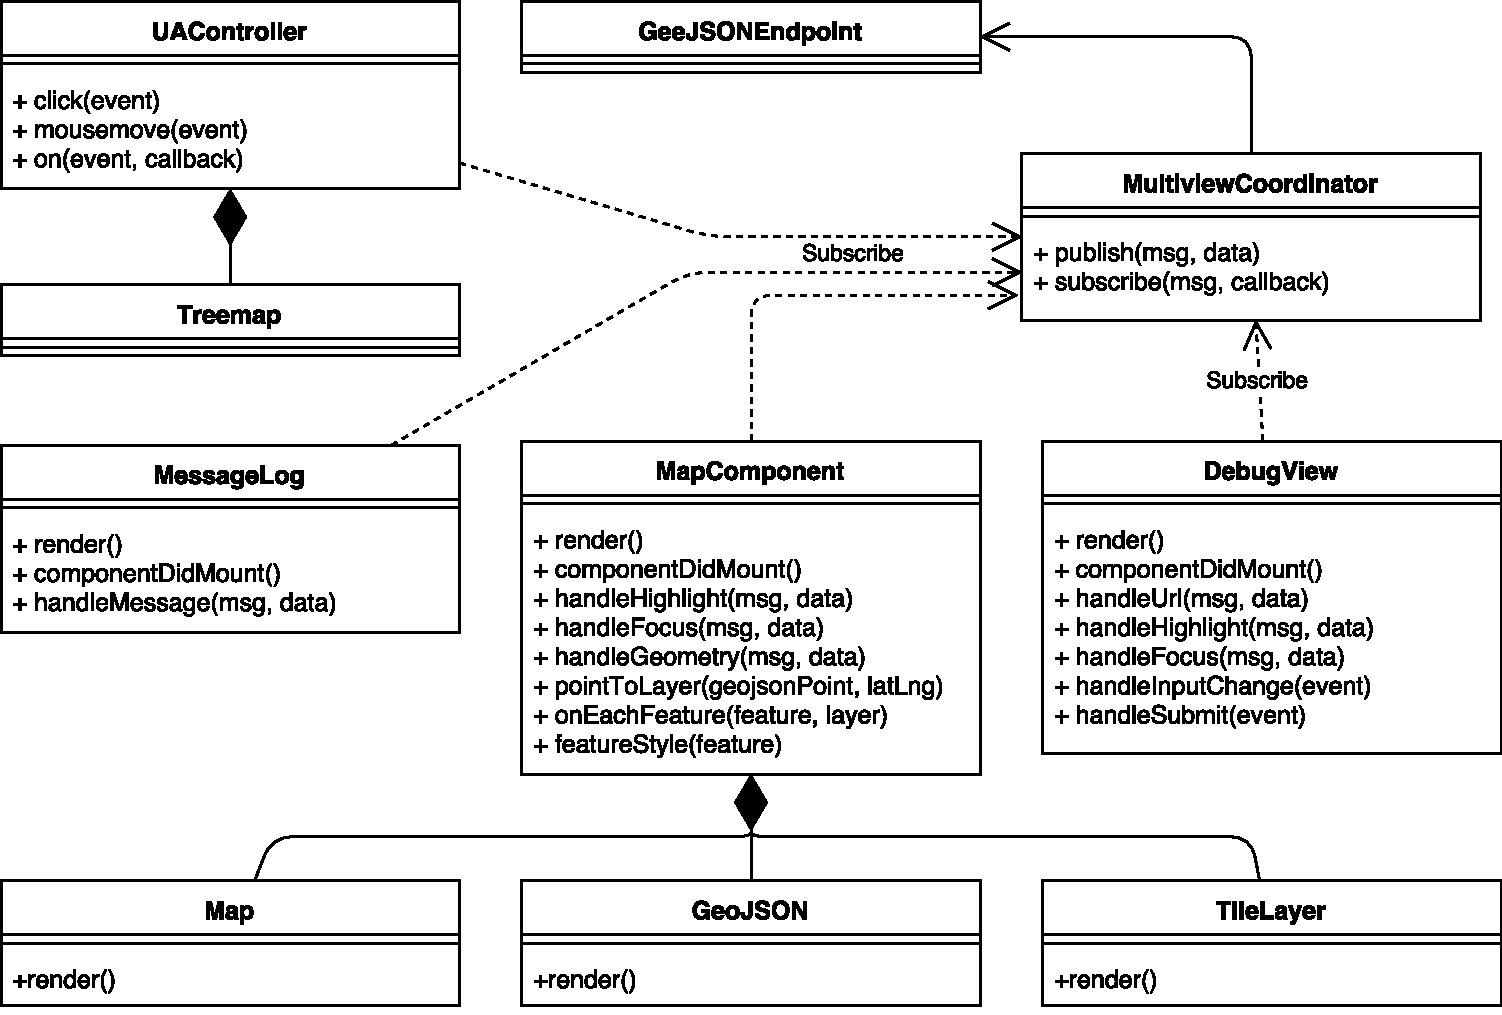
\includegraphics[width=\textwidth]{figures/implementation/Architecture.pdf}
\end{figure}

\section{Notifications}

The automatic update mechanism works only within the virtual DOM of React components.
Updates on view level need to be implemented manually.

In accordance to Chapter~\ref{sec:concept}, the class \attr{MultiviewCoordinator} implements the \attr{publish-subscribe} pattern for coordination and works as a broker for interactions across \cmvs{}.
To achieve this, it uses the JavaScript library \attr{PubSubJS} which is an topic-based, asynchronous implementation of the pattern.

Each view gets a reference to the coordinator, e.g. during initialization, and can subscribe to interactions as seen in Listing~\ref{lst:implementation:subscribe}.
\attr{PubSubJS} allows nested topics, so categories and purposes are encoded as nested strings.
A view can subscribe to a group of interactions, e.g.\ the group \attr{mcv.select} includes both \attr{mcv.select.highlight} and \attr{mcv.select.focus}.

Not only basic data types like numbers and strings can be published, as seen in Listing~\ref{lst:implementation:subscribe}, but also functions.
If an interaction of type \attr{filter} is published, it is not necessary to publish all filtered ids of entities explicitly.
Instead, the \attr{data} of the interaction can be a threshold function which, applied on an entity, returns whether or not the entity is filtered.

\lstinputlisting[
  label={lst:implementation:subscribe},
  caption={
    A simplified example how to subscribe to an interaction.
  }
]{listings/implementation/subscribe.js}


\section{MultiviewCoordinator}

As a central part of the implementation, the \attr{MultiviewCoordinator} is also used for certain performance optimizations and data integrity considerations.
Therefore, it is responsible to query geometry data.

Geometries are exchanged with \attr{GeoJSON}\footnotemark as data format.
\footnotetext{
  GeoJSON is a format for encoding a variety of geographic data structures~\cite{GeoJSON2017}.
  Based on JSON, it can represent simple geographic features like points, lines and areas and reserves a properties object for non-spatial attributes.
}

If the user selects a different data set, the \attr{url} of the GeoJSON endpoint changes and an update of the geometry data is required.
This behaviour is implemented by the \attr{MultiviewCoordinator} which observes all changes to the \attr{url} of the GeoJSON endpoint.
If the \attr{url} changes, the coordinator fetches geometry data, publishes a change of the geometries and all subscribed views can re-render.
This is also a performance optimization, as it reduces the number of requests to the \attr{GeoJSON} endpoint.

An example of these geometries can be seen in listing~\ref{lst:geojson:example}.
For convenience, the file includes the aggregated data in the \attr{properties} of each feature.
In this case the colors the shapes of the \tmap{} are based on the value of \attr{user_count_normalized}.
Each feature comes with a unique \attr{id} which is published when a user interacts with the feature.

\lstinputlisting[
  label={lst:geojson:example},
  caption={
    A GeoJSON example of a user distribution across German federal states, coordinates are omitted.
  }
]{listings/implementation/example.geojson}

\section{Adding the views to the DOM}

Adding the \gv{} to the DOM is straightforward.
Listing~\ref{lst:implementation:dom} shows an example how to use React's low-level API to render components inside the DOM.
It uses an id \attr{multiview-map-component} to reference a particular node in the HTML document in Listing~\ref{lst:implementation:dom-html} on line 3.
On lines 4 to 6 you can see the required JavaScript imports, i.e.\ two imports required by React and the compiled JavaScript application, which is called \attr{example.js}.

\lstinputlisting[
  label={lst:implementation:dom},
  lastline=12,
  caption={
    Example application written in TypeScript.
    Views can be added to the DOM individually.
    The implementation exposes convenient TypeScript declarations, here \attr{MultiviewCoordinator} and \attr{MapComponent} are imported.
  }
]{listings/implementation/dom.tsx}

\lstinputlisting[
  label={lst:implementation:dom-html},
  caption={
    This short HTML document shows how to render Views at a certain node inside the DOM.
    The id multiview-map-component is used as anchor.
  },
  language=HTML
]{listings/implementation/dom.html}

The reference implementation of the conceptual framework is written in \attr{TypeScript}\footnotemark.
The implementation exports typescript declaration and you can see an import of the classes \attr{MapComponent} and \attr{MultiviewCoordinator} on lines 1 to 3 in Listing~\ref{lst:implementation:dom}.
\footnotetext{
  TypeScript is a typed superset of JavaScript that compiles to plain JavaScript.
  It provides optional static typing, classes and interfaces and helps to reduce errors by raising type errors at compile time.
}


\section{Software patterns}\label{sec:implementation:patterns}
Figure~\ref{fig:implementation:sequence-diagram} shows how \cmvs{} can be automatically updated even if the environment lacks a native update-mechanism.

\begin{figure}[ht]
  \centering
  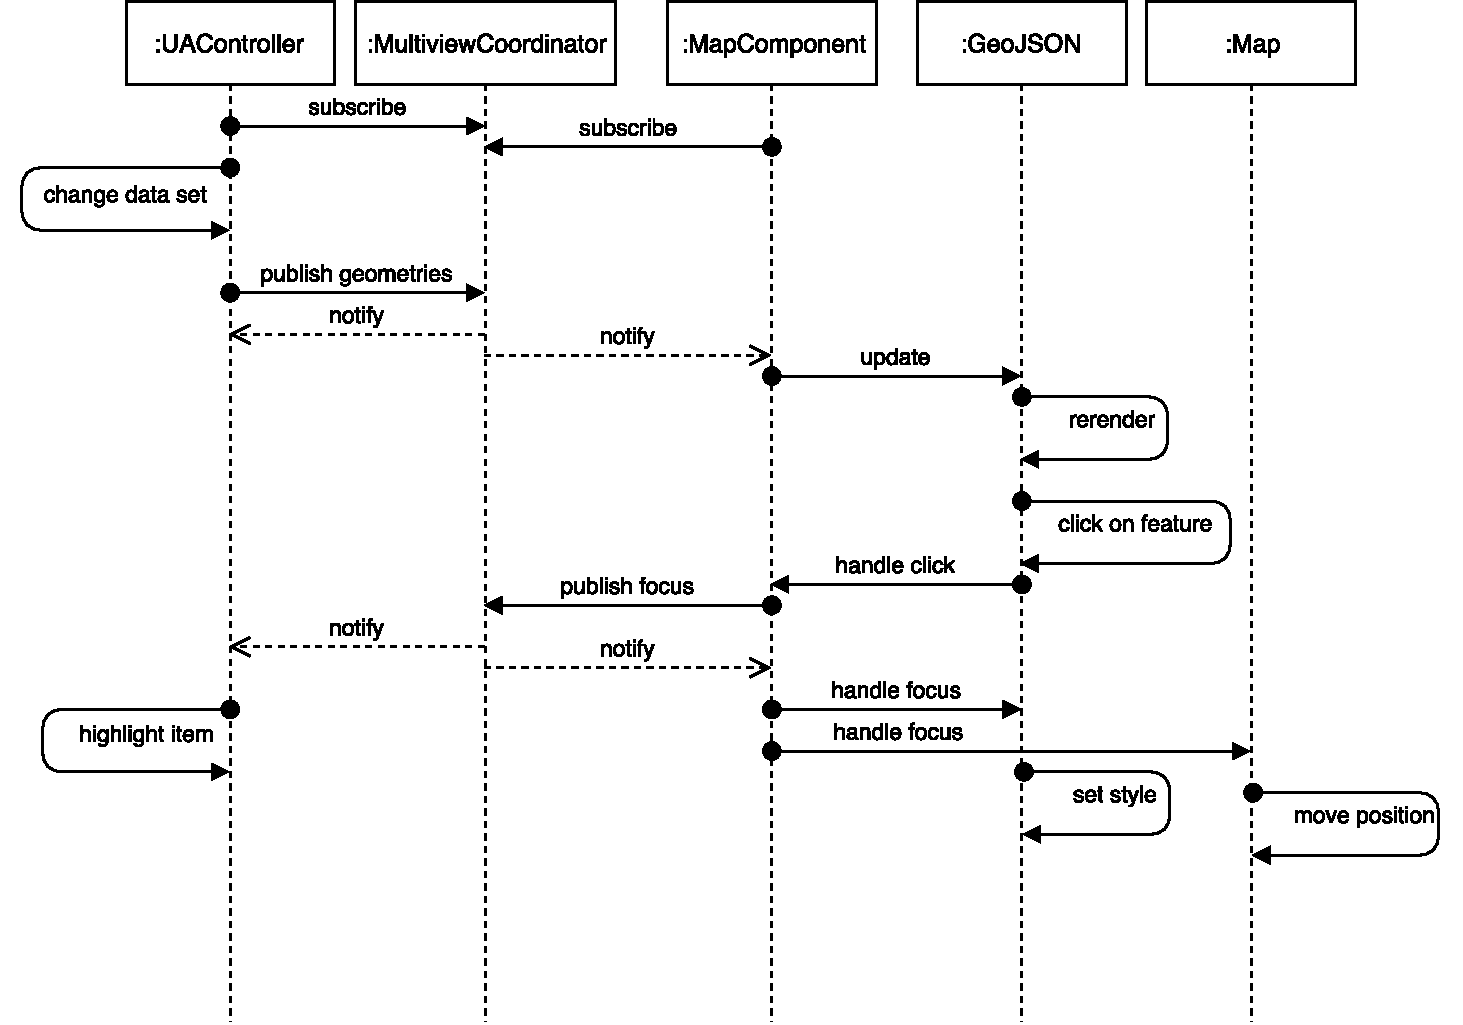
\includegraphics[width=\textwidth]{figures/implementation/SequenceDiagram}
  \caption{%
    The sequence diagram shows the notification of different components.
  The user first chooses a feature set and clicks on a polygon in the \gv{}.
  }\label{fig:implementation:sequence-diagram}
\end{figure}


\textbf{The Observer pattern} allows multiple \emph{observers} to react to changes of an observed state.
In our case, the observed state is the \attr{MultiviewCoordinator}.
Any change to the \attr{MultiviewCoordinator} will subsequently be broadcasted to all connected views.


\textbf{Publisher subscriber}
In our particular case we apply a special form of the observer pattern, the so called ``Publish-subscribe'' pattern\cite{Eugster2003}.
Publish-subscribe is a messaging pattern which is widely used in message queues.
In this scenario, senders of messages simply categorize their messages which will be consumed by subscribers of the category.
The scenario has very low coupling, publishers do not even need to know the existence of subscribers.

\textbf{Component pattern}
State-of-the-art JavaScript component frameworks like ReactJS and EmberJS follow the component pattern for the architecture of a single page web application.
The component pattern imposes a hierarchical structure on a website.
Each component is responsible for a task and may contain other components.
The components are joined at the root node of the page.

This pattern is very applicable to \cmvs{}.
The different views of \cmvs{} share state, i.e.\ the feature, that is currently highlighted or the applied filter on the data.
So the views are components and their closest common ancestor is the \cmv{} itself, controlling state and passing user interaction down to it's children.

\textbf{Actions up --- Data down}

Version 2.0 of Ember introduced a common phrase how to use this pattern effectively: ``Data down, actions up''\cite{Emberigniter2017}
In the domain of \cmvs{} actions would mean user interactions, e.g.\ a click on a feature.
The action will notify the controlling \cmv{} component.
Actions may change data, and the changes will be passed to to all dependent views.
These views are then re-rendered.

Examples for the kind of data that might trigger a re-rendering of a view:
\begin{itemize}
  \item
    The selected feature or a list of selected features
  \item
    A list of thresholds for certain features as a filter
\end{itemize}


\section{Map Component}

The geographical visualization is implemented as a \attr{Map} component of the React Leaflet library.
Listing \ref{lst:implementation:render} shows the \attr{render} method of the component.

\lstinputlisting[
  label={lst:implementation:render},
  caption={\attr{render} method of the Map component of the geographical visualization}
]{listings/implementation/render.tsx}

The \attr{render} method is the only required method of a React component.
It will be invoked on the initial rendering of the component of the \attr{DOM} and on every update of the component's properties.
React's templating language ``\attr{JSX}'' allows to nest other child components into the React parent component.
In this case the \attr{Map} component includes a \attr{TileLayer} \attr{GeoJSON} component from the \attr{react-leaflet} library.
This library conveniently provides ``React components for Leaflet maps.''~\cite{ReactLeaflet2017}.

\subsection{GeoJSON Component}

The \attr{GeoJSON} component is provided by the \attr{Map} component with a couple of properties:
It gets a
\begin{enumerate*}[label=(\arabic*)]
  \item
    geojsonURL as well as a
  \item
    geojson as data attribute. Furthermore a couple of callbacks is passed into the child component, including
  \item
    featureStyle,
  \item
    pointToLayer and
  \item
    onEachFeature.
\end{enumerate*}

This way, the parent \attr{Map} component controls the data flow and without a \attr{geojson} object, no polygons are placed on the map.
A changed \attr{geojsonURL} will always update the child component as it is used a \attr{key} on the \attr{GeoJSON} component.
The callbacks passed into the \attr{GeoJSON} component control the visual representation of each polygon and they add event handlers for a mouse click or a mouse move on each polygon.
Listing \ref{lst:implementation:onEachFeature} shows the event handlers added to the map.

\lstinputlisting[
  label={lst:implementation:onEachFeature},
  caption={\attr{onEachFeature} callback, adding handlers for mouse events}
]{listings/implementation/onEachFeature.tsx}

First we cache all layers in the internal state of the \attr{Map} component.
On each \attr{mouseover} event, the \attr{id} of the feature is published as \attr{mcv.select.highlight} interaction.
A \attr{click} event is distinguished if the control key is pressed or not.
In the latter case, the id of the feature is either added or removed from the list of focused ids and then the list of focused ids is published as \attr{mcv.select.focus} interaction.

\lstinputlisting[
  label={lst:implementation:featureStyle},
  caption={\attr{featureStyle} callback, configuring the visual appearance depending on the currently highlighted or focused feature ids}
]{listings/implementation/featureStyle.tsx}

The \attr{featureStyle} in Listing \ref{lst:implementation:featureStyle} method is very straightforward.
If the feature is currently focused, the \attr{fillColor} of the polygon is red, otherwise blue.
Likewise, if the feature is currently highlighted, the polygon has a white, solid stroke.

\lstinputlisting[
  label={lst:implementation:pointToLayer},
  caption={\attr{pointToLayer} callback, if a feature of \attr{GeoJSON} has a point geometry, it will be shown as a circle}
]{listings/implementation/pointToLayer.tsx}

Finally, we configure how to display point geometries in callback \attr{poinToLayer}.
Since normal markers do not have a configurable color and style, we instruct the \attr{GeoJSON} component to render a \attr{CircleMarker} for each point geometry instead.
This way, the same options of \attr{featureStyle} can be applied to both point and area geometries.





	\chapter{Evaluation}\label{sec:evaluation}
\todo[inline]{How and what can we evaluate?}
\todo[inline]{The performance?}
\todo[inline]{The flexibility?}
\section{Use case}\label{sec:use-case}
\todo[inline]{No section without text}

\subsection{Data Sets}
For our uses cases, we have two different data sets:
One data set consists of a user ranking of public broadcasting in Germany, i.e.\ entities, mostly TV and radio broadcasts, are liked or disliked by people.
This data is public data and can be used by media researchers of broadcasting corporations but also targets media journalists and the general audience.
The other set, called \riso{}, consists of statistical data from various German administrations and is used by the authorities for urban planning and policy strategies.

Both data sets share some characteristics.
The administrative data connects certain features with certain regions of Germany.
As Germany is a federal state, larger regions consist of many other smaller regions.

The second one consists of user data that was collected through a web application called \rufu{}.

\subsubsection{RISO}

The \riso{} data base is used in by local authorities to get insights about governmental KPIs to assist local and regional decision making.
It is a relational database and a part of the data base schema is shown as an ER diagram in Figure~\ref{fig:data:riso}.

\begin{figure}[h!]
  \centering
  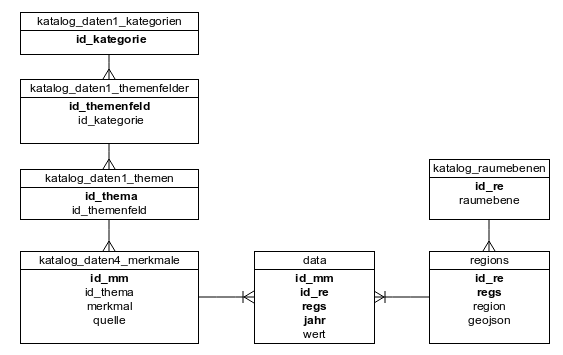
\includegraphics[width=\textwidth]{images/riso}
  \caption{Part of the \riso{} database schema. Primary keys are set in bold.}\label{fig:data:riso}
\end{figure}

The largest table is called \attr{data} with approximately 10,466,600 records, which holds all values along with the survey date.
\paragraph{Features}
This data is connected to a feature table through a foreign key called \attr{id_mm}.
In the feature table we can find the description for every referenced feature, e.g.\ population density, working population in agriculture, education spending.
The \riso{} system groups all features in a 4-level hierarchy:
\begin{enumerate}
  \item
    \attr{katalog_daten_1_kategorien}
  \item
    \attr{katalog_daten_2_themenfelder}
  \item
    \attr{katalog_daten_3_themen}
  \item
    \attr{katalog_daten_4_merkmale}
\end{enumerate}
The actual features table is the last one in the list.
At the lowest level within the hierarchy, this is the largest table with 1234 records.


\paragraph{Regions}
On the other side, the geographical data is stored in the \attr{regions} table.
The geometry data for each region is stored in the \attr{geojson} column and as the name suggests, the data type is a \attr{geojson}.
The foreign keys that connect the tables \attr{data} and \attr{regions} are called \attr{id_re} and \attr{regs}.
Unlike the feature table, the regions are grouped through the \attr{id_re} that indicates the hierarchy level.
So the values of the \attr{id_re} column denominate the level of the hierarchy.
E.g.\ a region with a \attr{id_re} of $1$ is a federal state of Germany, a region with id $13$ is a constituency.
A textual description for the hierarchy level can be found in the \attr{katalog_raumebenen} table in column \attr{raumebene}.
Both column \attr{id_re} and \attr{regs} belong to the primary key of the regions table, so there will never be two regions on the same hierarchy level with the same \attr{regs} id.

\paragraph{Characteristics}
As we can see, the schema of the \riso{} database follows a rather denormalized approach.
The schema does not make a lot of assumptions regarding the input data.
It allows to add data of arbitrary size, features and completeness as long as there is some kind of numerical data associated with some kind of geographical unit.
This approach is suitable for a data base that incorporates data from different sources, as it is the case with the \riso{} data base.


\subsubsection{\rufu{}}
Unlike the \riso{} database, the data base of \rufu{} is used as persistence layer.
For that reason the data base schema follows the requirements of a web application in production.

As outlined in Section~\ref{sec:outline} \rufu{} is an evaluation platform for public broadcasting in Germany.
First, users vote on broadcasts, i.e.\ they decide if they want to support broadcast or if they do not want to support.
As a next step, user can define a weighting by distributing a virtual, monthly budget among the chosen broadcasts.

Figure~\ref{fig:data:rundfunk} shows the data base schema of the application.
A \attr{user} is connected to \attr{broadcast} through a \attr{selection}.
If the \attr{user} supports some a broadcast, the \attr{response} on the given \attr{selection} will be `positive'.
If the \attr{user} does not wish to support a \attr{broadcast}, the \attr{response} will be `neutral'.
The \attr{user} can allocate virtual money to supported broadcasts.
The money will be stored in the column \attr{amount} of the \attr{selection}.
The sum of all amounts for one user will never exceed the virtual budget of 17.50€.

\begin{figure}[h!]
  \centering
  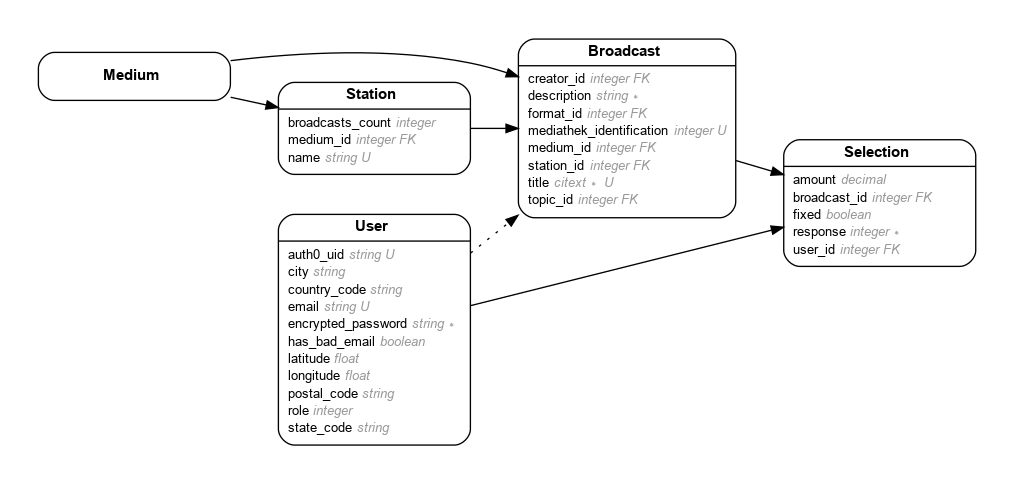
\includegraphics[width=\textwidth]{images/er}
  \caption{Database schema of the \rufu{} app}\label{fig:data:rundfunk}
\end{figure}

\paragraph{Features}
We have both numerical as well as nominal features.
A numerical feature could be the number of supporters from an area in Germany.
A nominal feature could be a list of the most supported broadcasts from an area in Germany.
Numerical and nominal features can be combined, so we could request for every region, a distribution of the desired expenditure for radio, TV, online and other broadcasts.

\paragraph{Regions}
\rufu{} stores the geometry for each region in \attr{geojson} files.
These files hold a \attr{FeatureCollection}.
Every \attr{Feature} is a region, the identifier is stored as a property.
We merge the geometry data with features for every request.
To be precise: We get all the user data, group it by the identifier \attr{state_code} and merge it with the geometry in the \attr{geojson}.

\paragraph{Characteristics}
The data base schema is a result of the specific requirements of the persistence layer.
Changes in the source code may require a migration of the data base schema.

However, we can ask a lot of questions already with common data base queries or standard data analysis tools:
\begin{enumerate}
  \item
    How does the actual support of a broadcast compare to the average support of a broadcast?
  \item
    What are the most popular broadcasts in Berlin?
  \item
    What is the desired ratio of genres of supported broadcasts? How important is education compared to sport?
  \item
    How does the support of a broadcast change over time?
  \item
    According to the user ranking, which broadcasts are similar to each other?
\end{enumerate}


\subsection{Existing Interactions}
We will now classify the implemented interactions of our two applications according to the classification by \textcite{Yi2007} in Section~\ref{sec:related-work:categories}.

\paragraph{In our \visan{}} possible interactions can be categorized into the classes \emph{select}, \emph{explore}, \emph{reconfigure}, \emph{encode} and \emph{filter}.
As seen in Figure~\ref{fig:analysis:interaction:existing} the user can \emph{select} one item in the view by clicking on it.
The user can reveal a tooltip showing the item properties by hovering with the mouse on the item, which is another \emph{selection}.
The user can \emph{explore} the map in the usual manner:
If the user drags with the mouse on the map, a panning operation is performed with the viewpoint focused on Germany, i.e.\ the camera moves around like a turntable.
The zoom factor can be changed by scrolling on the canvas of the map.
\emph{Encode} and \emph{reconfigure} techniques are performed through the menu on the left side:
Under the ``features'' tab, the user can \emph{reconfigure} different data sets and the displayed diagram, e.g.\ a tree map visualization based on the geometry shape, cubes or voronoi regions.
The tab ``Dimensions'' allows the user to \emph{encode} properties of a data set to visual attributes, e.g.\ the height, color and texture of an item.
The tab ``Filter'' can be used to reduce the displayed data set along a range of continuous values.
Figure~\ref{fig:analysis:interaction:existing:filter} shows the range of visible values in the left menu.
When the user drags the slider, the items in the map on the right side are updated interactively.

\begin{figure}[h!]
  \centering
  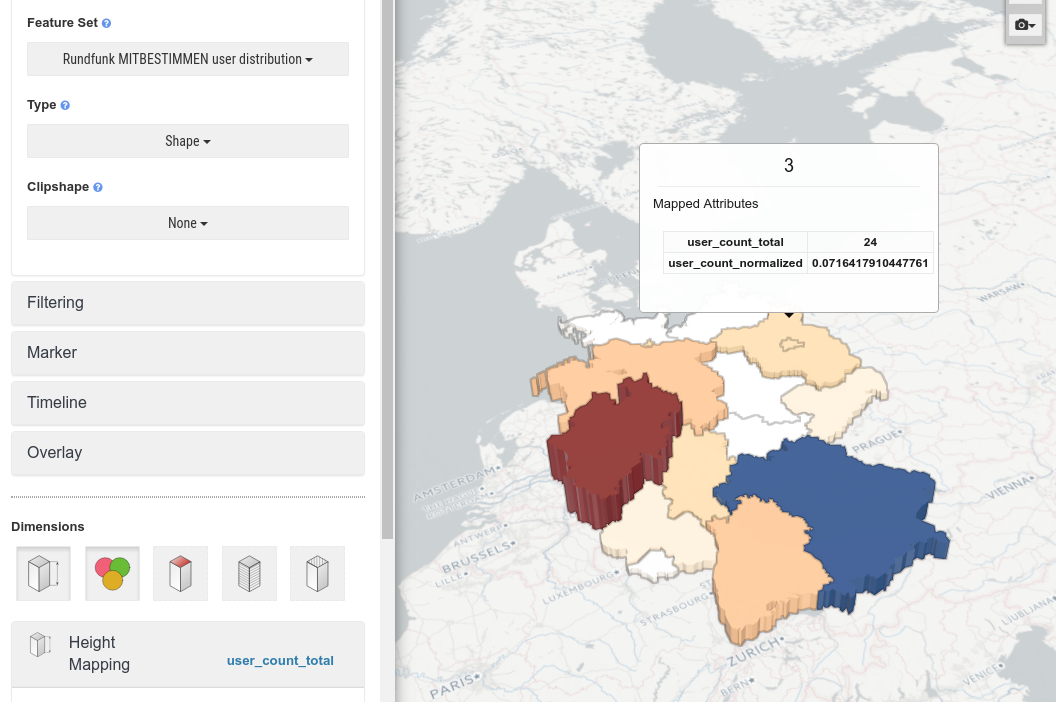
\includegraphics[width=\textwidth]{images/existing-interactions.png}
  \caption{%
    Items can be highlighted with a click, Bavaria is currently highlighted.
    A mouse over reveals a tooltip showing item properties.
    The menu on the left side allows to change the data set and the specific base visualization.
  }\label{fig:analysis:interaction:existing}
\end{figure}

\begin{figure}[h!]
  \centering
  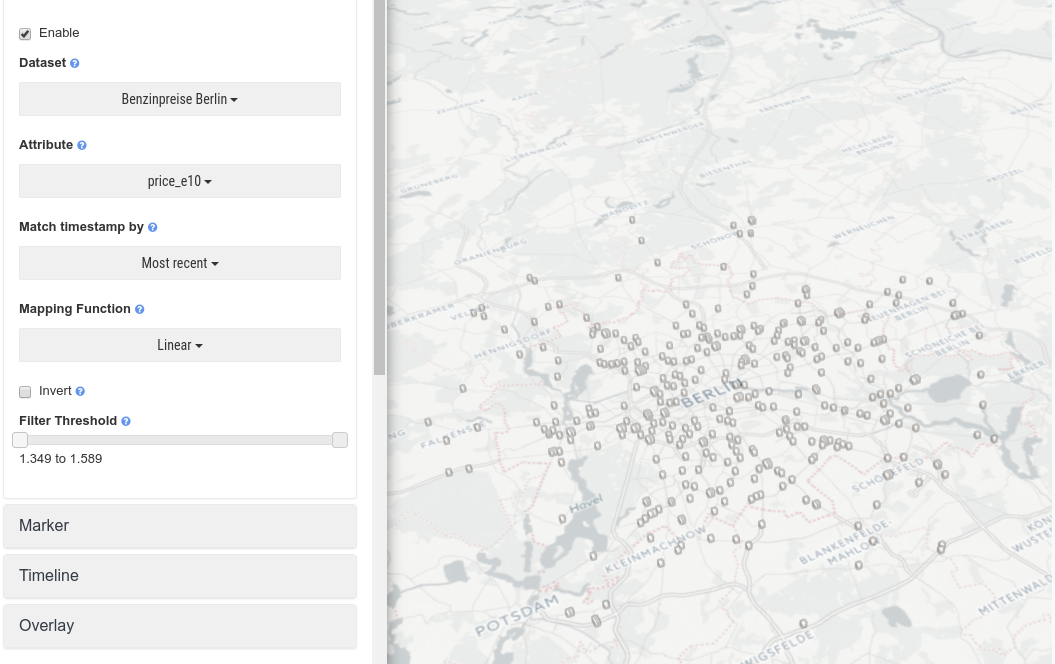
\includegraphics[width=\textwidth]{images/existing-interactions-filter.png}
  \caption{%
    Only gas stations with a price for E10 within 1.349 Euro and 1.589 Euro are displayed in the map
  }\label{fig:analysis:interaction:existing:filter}
\end{figure}

\subsection{Planned Interactions}
We have a focus on coordinated multiple views consisting of a tree map and a geographical map.
Let's have some examples how an interaction between a \tmap{} and a \map{} might work:

    \begin{enumerate}
      \item
        User selects a feature set from the drop down in the menu. This will trigger a \emph{Reconfigure} interaction. A data set consisting of all features and their ids, geometries and metadata is transferred. The receiving components are both the \tmap{} and the \map{} which will rerender the entire visualization.
      \item
        User hovers with a mouse over a polygon in the \map{}. This will trigger a \emph{Select} interaction. The data is a single feature id that will be transferred to the \tmap{}, which will change the color of an box.
      \item
        Rotate or zoom the \tmap{}. This will also rotate or zoom the \map{}. The interaction would fall into \emph{Explore} and the shared information is the orientation of the camera and the zoom level.
      \item
        A click in the \tmap{} will trigger an \emph{Explore} interaction. The data is a single feature id sent to the \map{}. The map will center the viewport on the center of geometry of the respective feature.
      \item
        The user selects many features at once in the \map{} by dragging a rectangle. The ids of all features within the rectangle are sent to the \tmap{}. All features will be highlighted with a different color, which is therefore a \emph{Select} interaction.
      \item
        \emph{Reconfigure} the layouting of the \tmap{} by choosing a different hierarchy level. This increased granularity may lead to an increased granularity in the \map{}, e.g.\ show postal codes instead of federal states. The changed data are additional items, that are nested in the former items.
      \item
        \emph{Encode} the \tmap{} by a different attribute mapping like color, height or texture. If the \map{} has no geometry data that defines the shape of a feature, it can also display a larger point marker.
      \item
        Apply a \emph{Filter} and reduce the data set by choosing only items with metadata beyond a certain treshold. The reduced data leads to a full re-render of all data visualizations. The message contains the updated item list
  \item
    Show a \emph{Connect} by highlighting boxes of the same subtree in the \tmap{}. The respective connected items would be highlighted in the \map{} as well. Here the data is a relation between items.
    \end{enumerate}
\todo[inline]{What are the key interactions in our use case?}


	\chapter{Conclusion and Future Work}\label{sec:conclusion}
\todo[inline]{Did we achieve our goals?}
\todo[inline]{Is the concept sane in regarding the implementation?}

\todo[inline]{List stuff which was not accomplished in this master thesis}



	\clearpage
%	\printglossary[type=\acronymtype,style=modsuper]
	\printbibliography{}
	% \input{chapters/appendix}
	\chapter*{Declaration of Authorship}
\thispagestyle{empty}   
I certify that I have written the paper by myself and that I have not  
used other than the stated resources and means.
% I certify that the work presented here is, to the best of my  
% knowledge and belief, original and the result of my own  
% investigations, except as acknowledged, and has not been submitted,  
% either in part or whole, for a degree at this or any other University.
\\
\\
\\
\\
\\
Potsdam, \today
\\
\\
\\
\\
\AUTHOR


\end{document}
